% Change numbering of tables and figures
\setcounter{table}{0}
\renewcommand{\thetable}{A\arabic{table}}
\setcounter{figure}{0}
\renewcommand{\thefigure}{A\arabic{figure}}

\section{Figures and Tables from Chapter \ref{sec:real-data}}

\begin{figure}[h!]
    \centering
    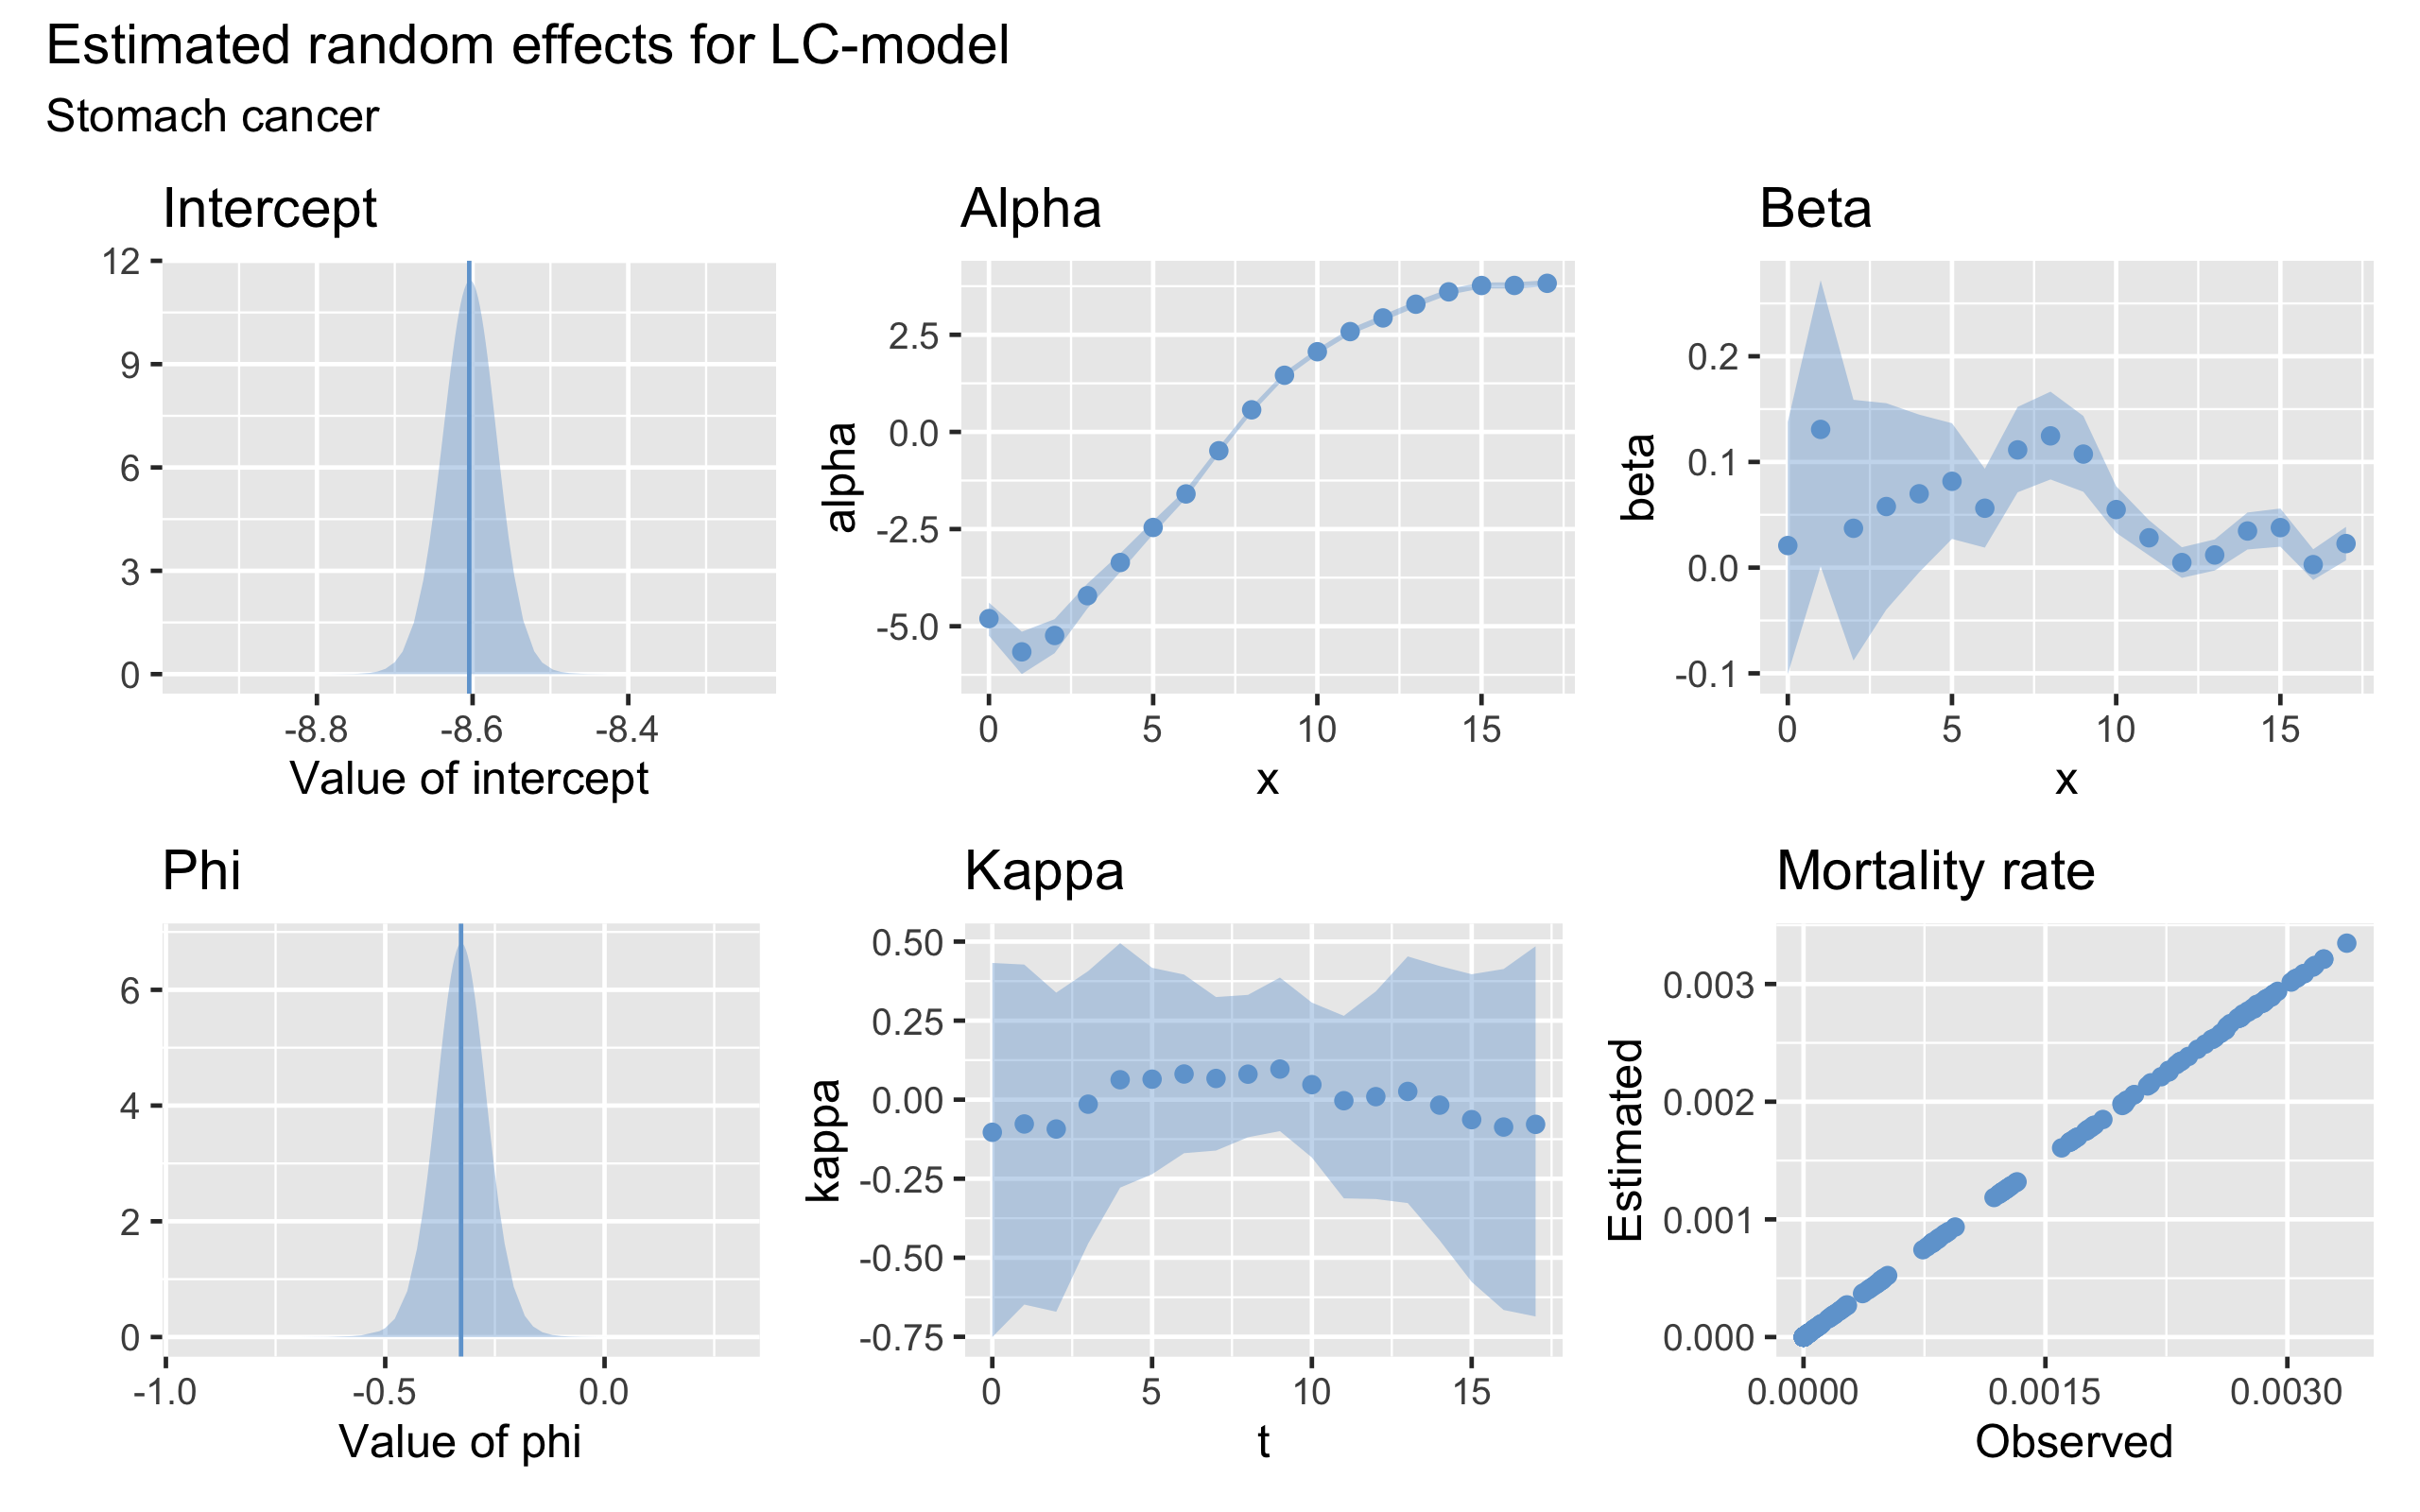
\includegraphics[width=0.85\linewidth]{real-data/real-data-univariate/Figures/uv-full-data-lc-s.png}
    \caption{The estimation results from fitting the LC-model to the stomach cancer data. The layout of the plots is similar to that of Figure \ref{fig:uv-full-data-LC-l}.}
    \label{fig:uv-full-data-LC-s}
\end{figure}

\begin{figure}[h!]
    \centering
    \begin{subfigure}[b]{.75\linewidth}
        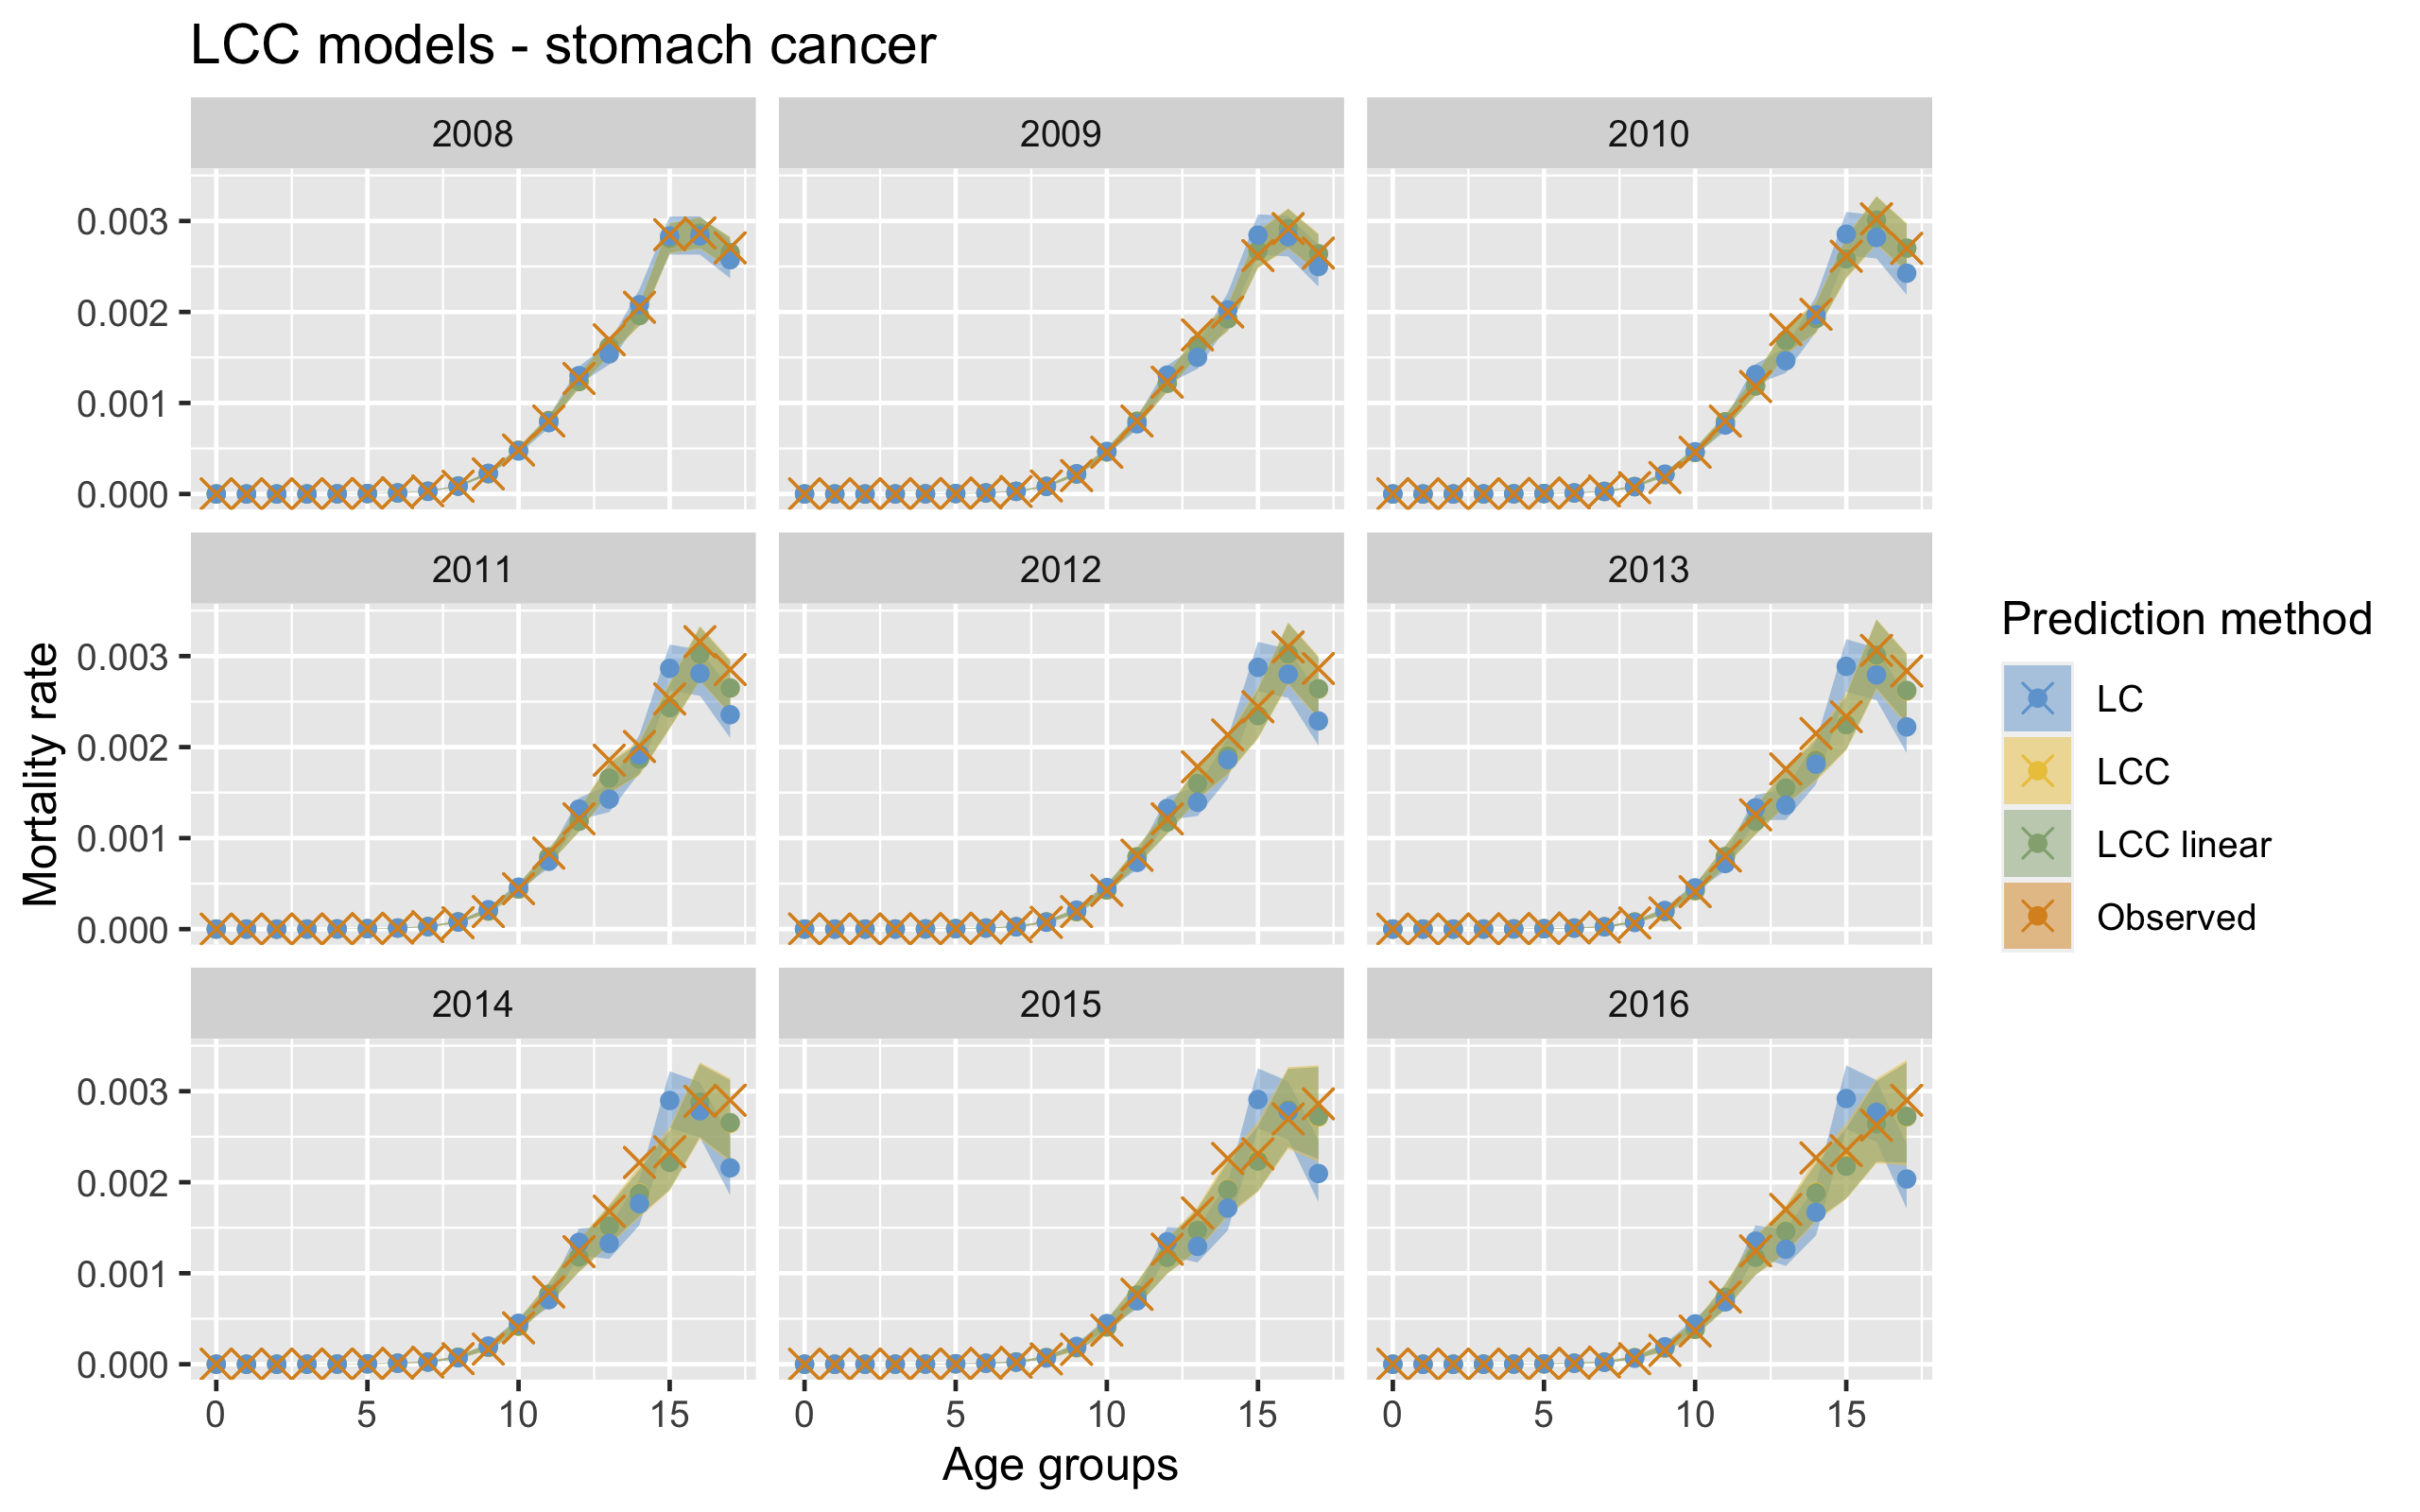
\includegraphics[width=\linewidth]{real-data/real-data-univariate/Figures/univariate-LCC-by-age-stomach.png}
        \caption{The prediction results plotted for each of the years that were predicted, with the age groups along the horizontal axis.}
        \label{fig:uv-LCC-stomach-top}
    \end{subfigure}
    
    \begin{subfigure}[b]{.75\linewidth}
        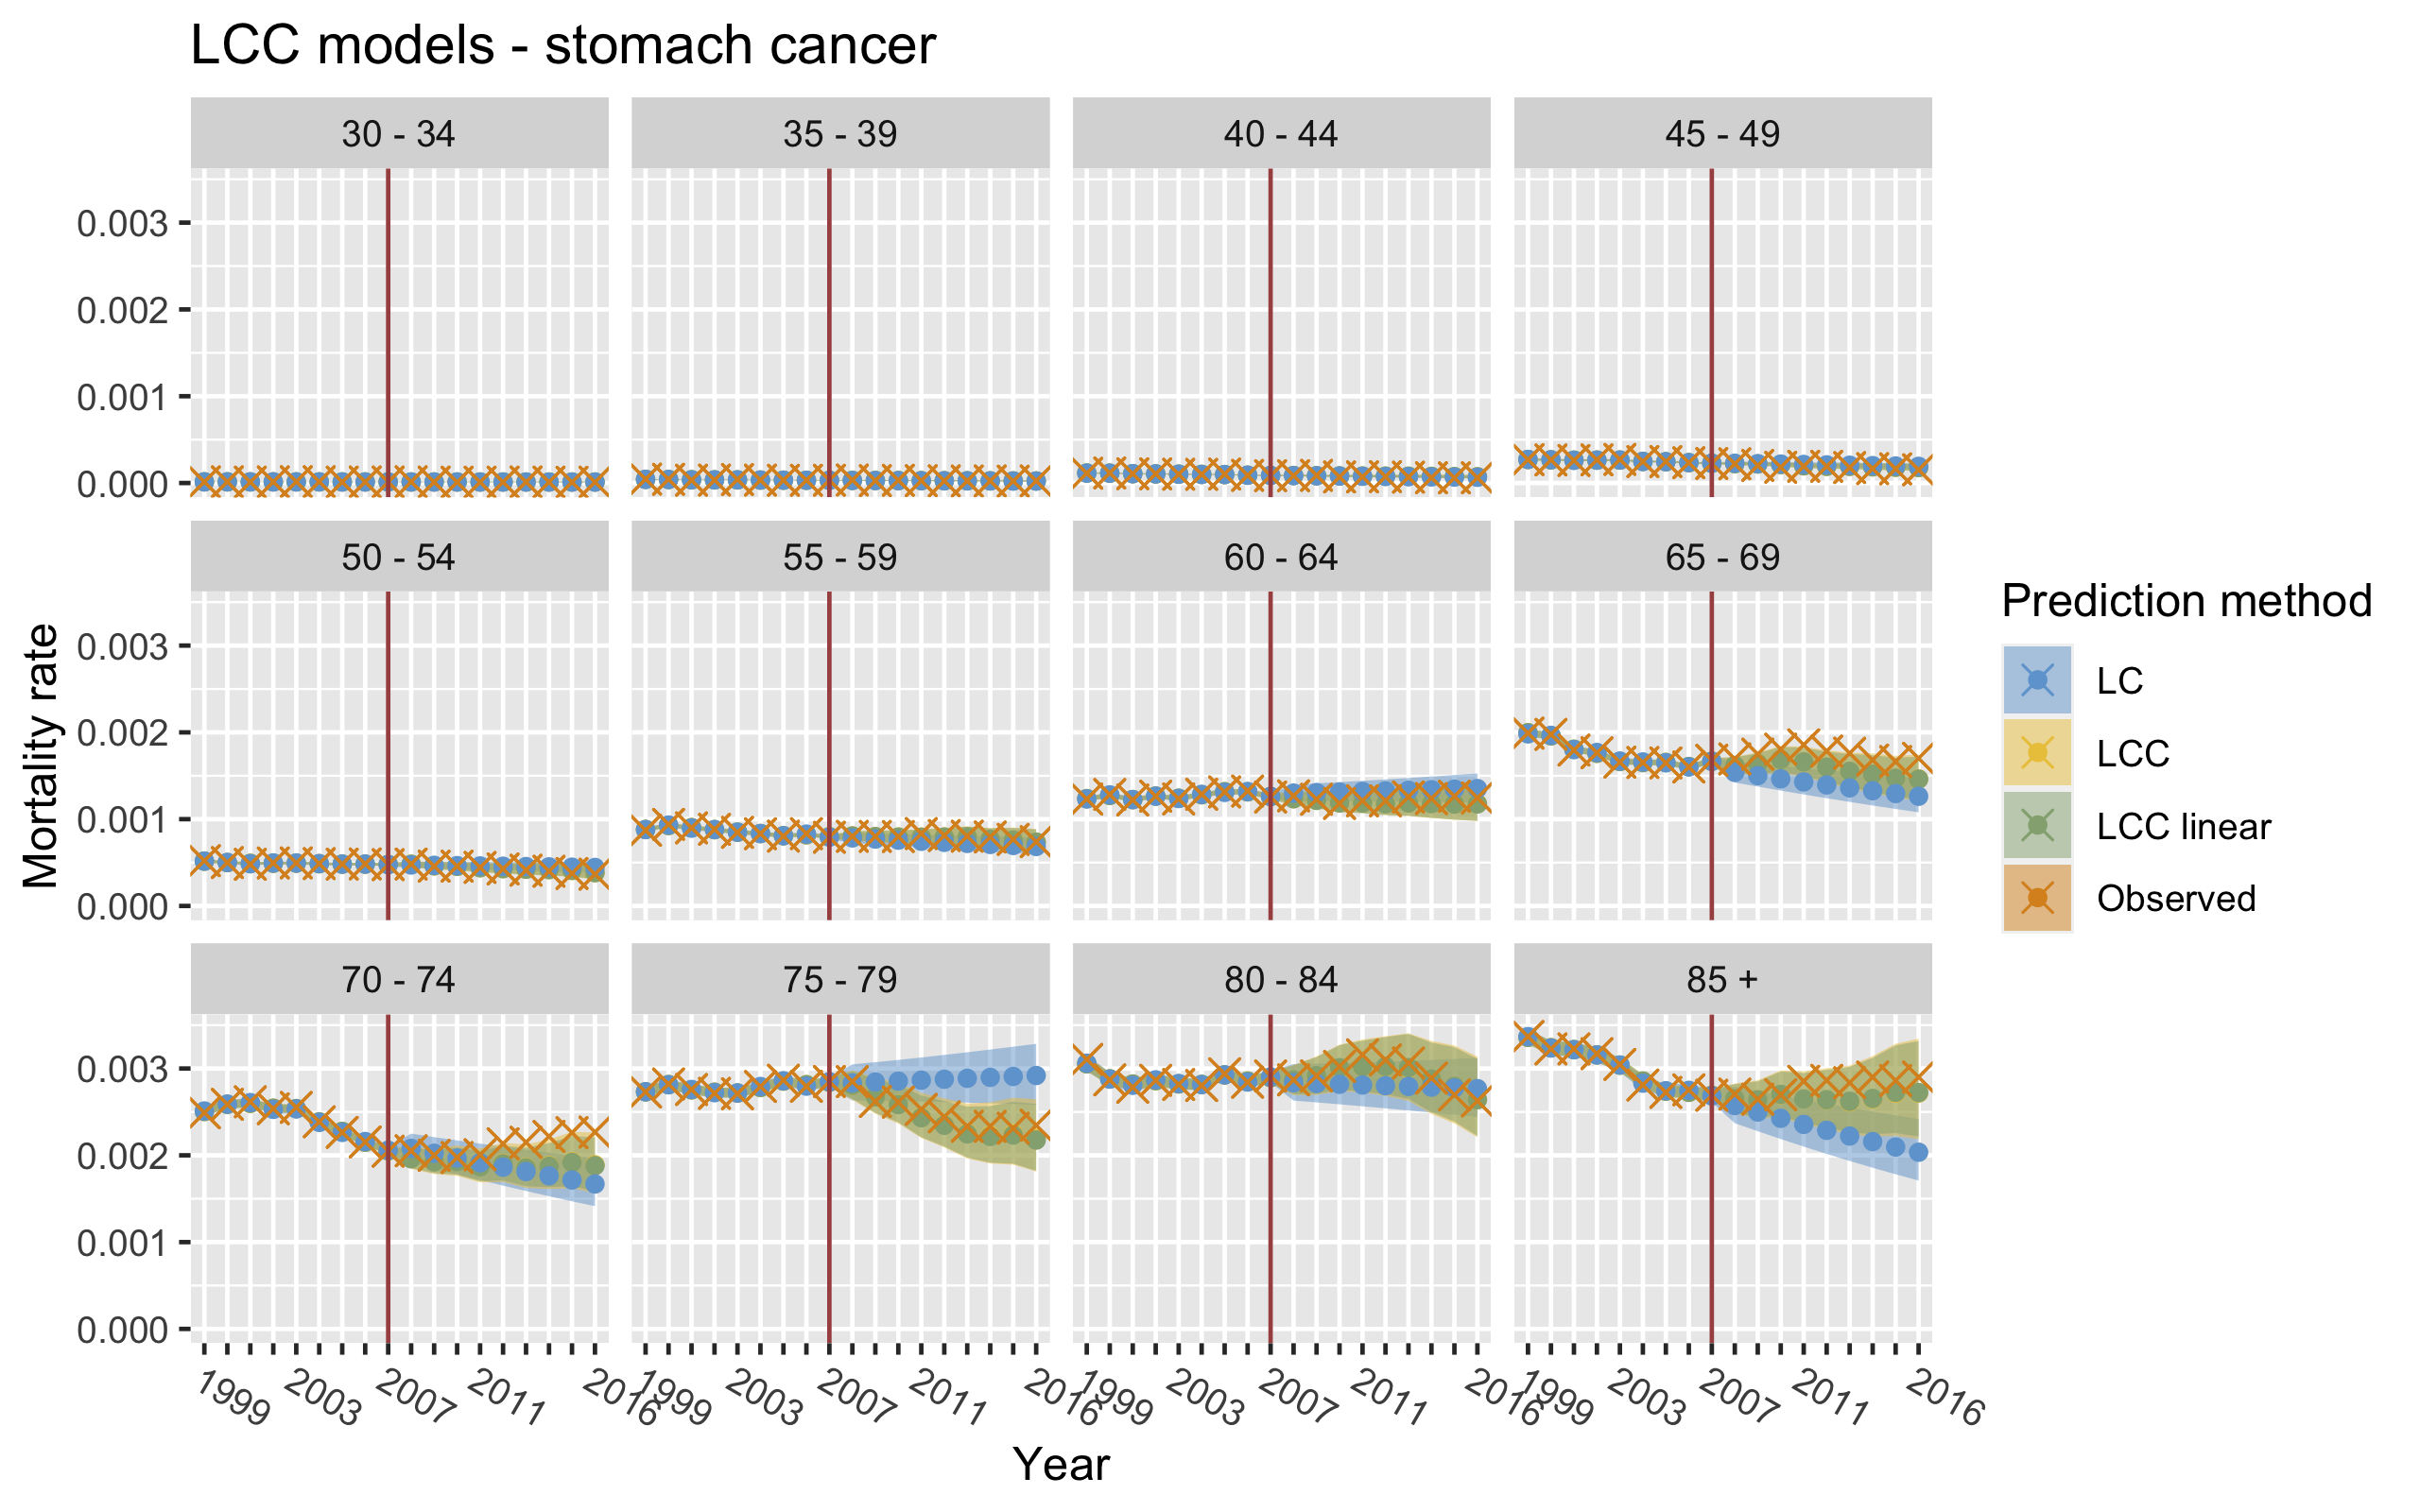
\includegraphics[width=\linewidth]{real-data/real-data-univariate/Figures/univariate-LCC-by-period-stomach.png}
        \caption{The prediction results plotted for each age group that are 30 years and older, with the calendar years along the horizontal axis. The red line marks the beginning of the predicted periods.}
        \label{fig:uv-LCC-stomach-bottom}
    \end{subfigure}
    \caption{The mean values and the 95\% confidence bounds of the predicted expected stomach cancer mortality rates produced by inference with three Lee-Carter types of models on data of German stomach cancer (circles), together with the corresponding observed mortality rates $Y_{x,y}^{\text{stomach}}$ (crosses).}
    \label{fig:uv-LCC-stomach}
\end{figure}

\begin{figure}[h!]
    \centering
    \begin{subfigure}[b]{.75\linewidth}
        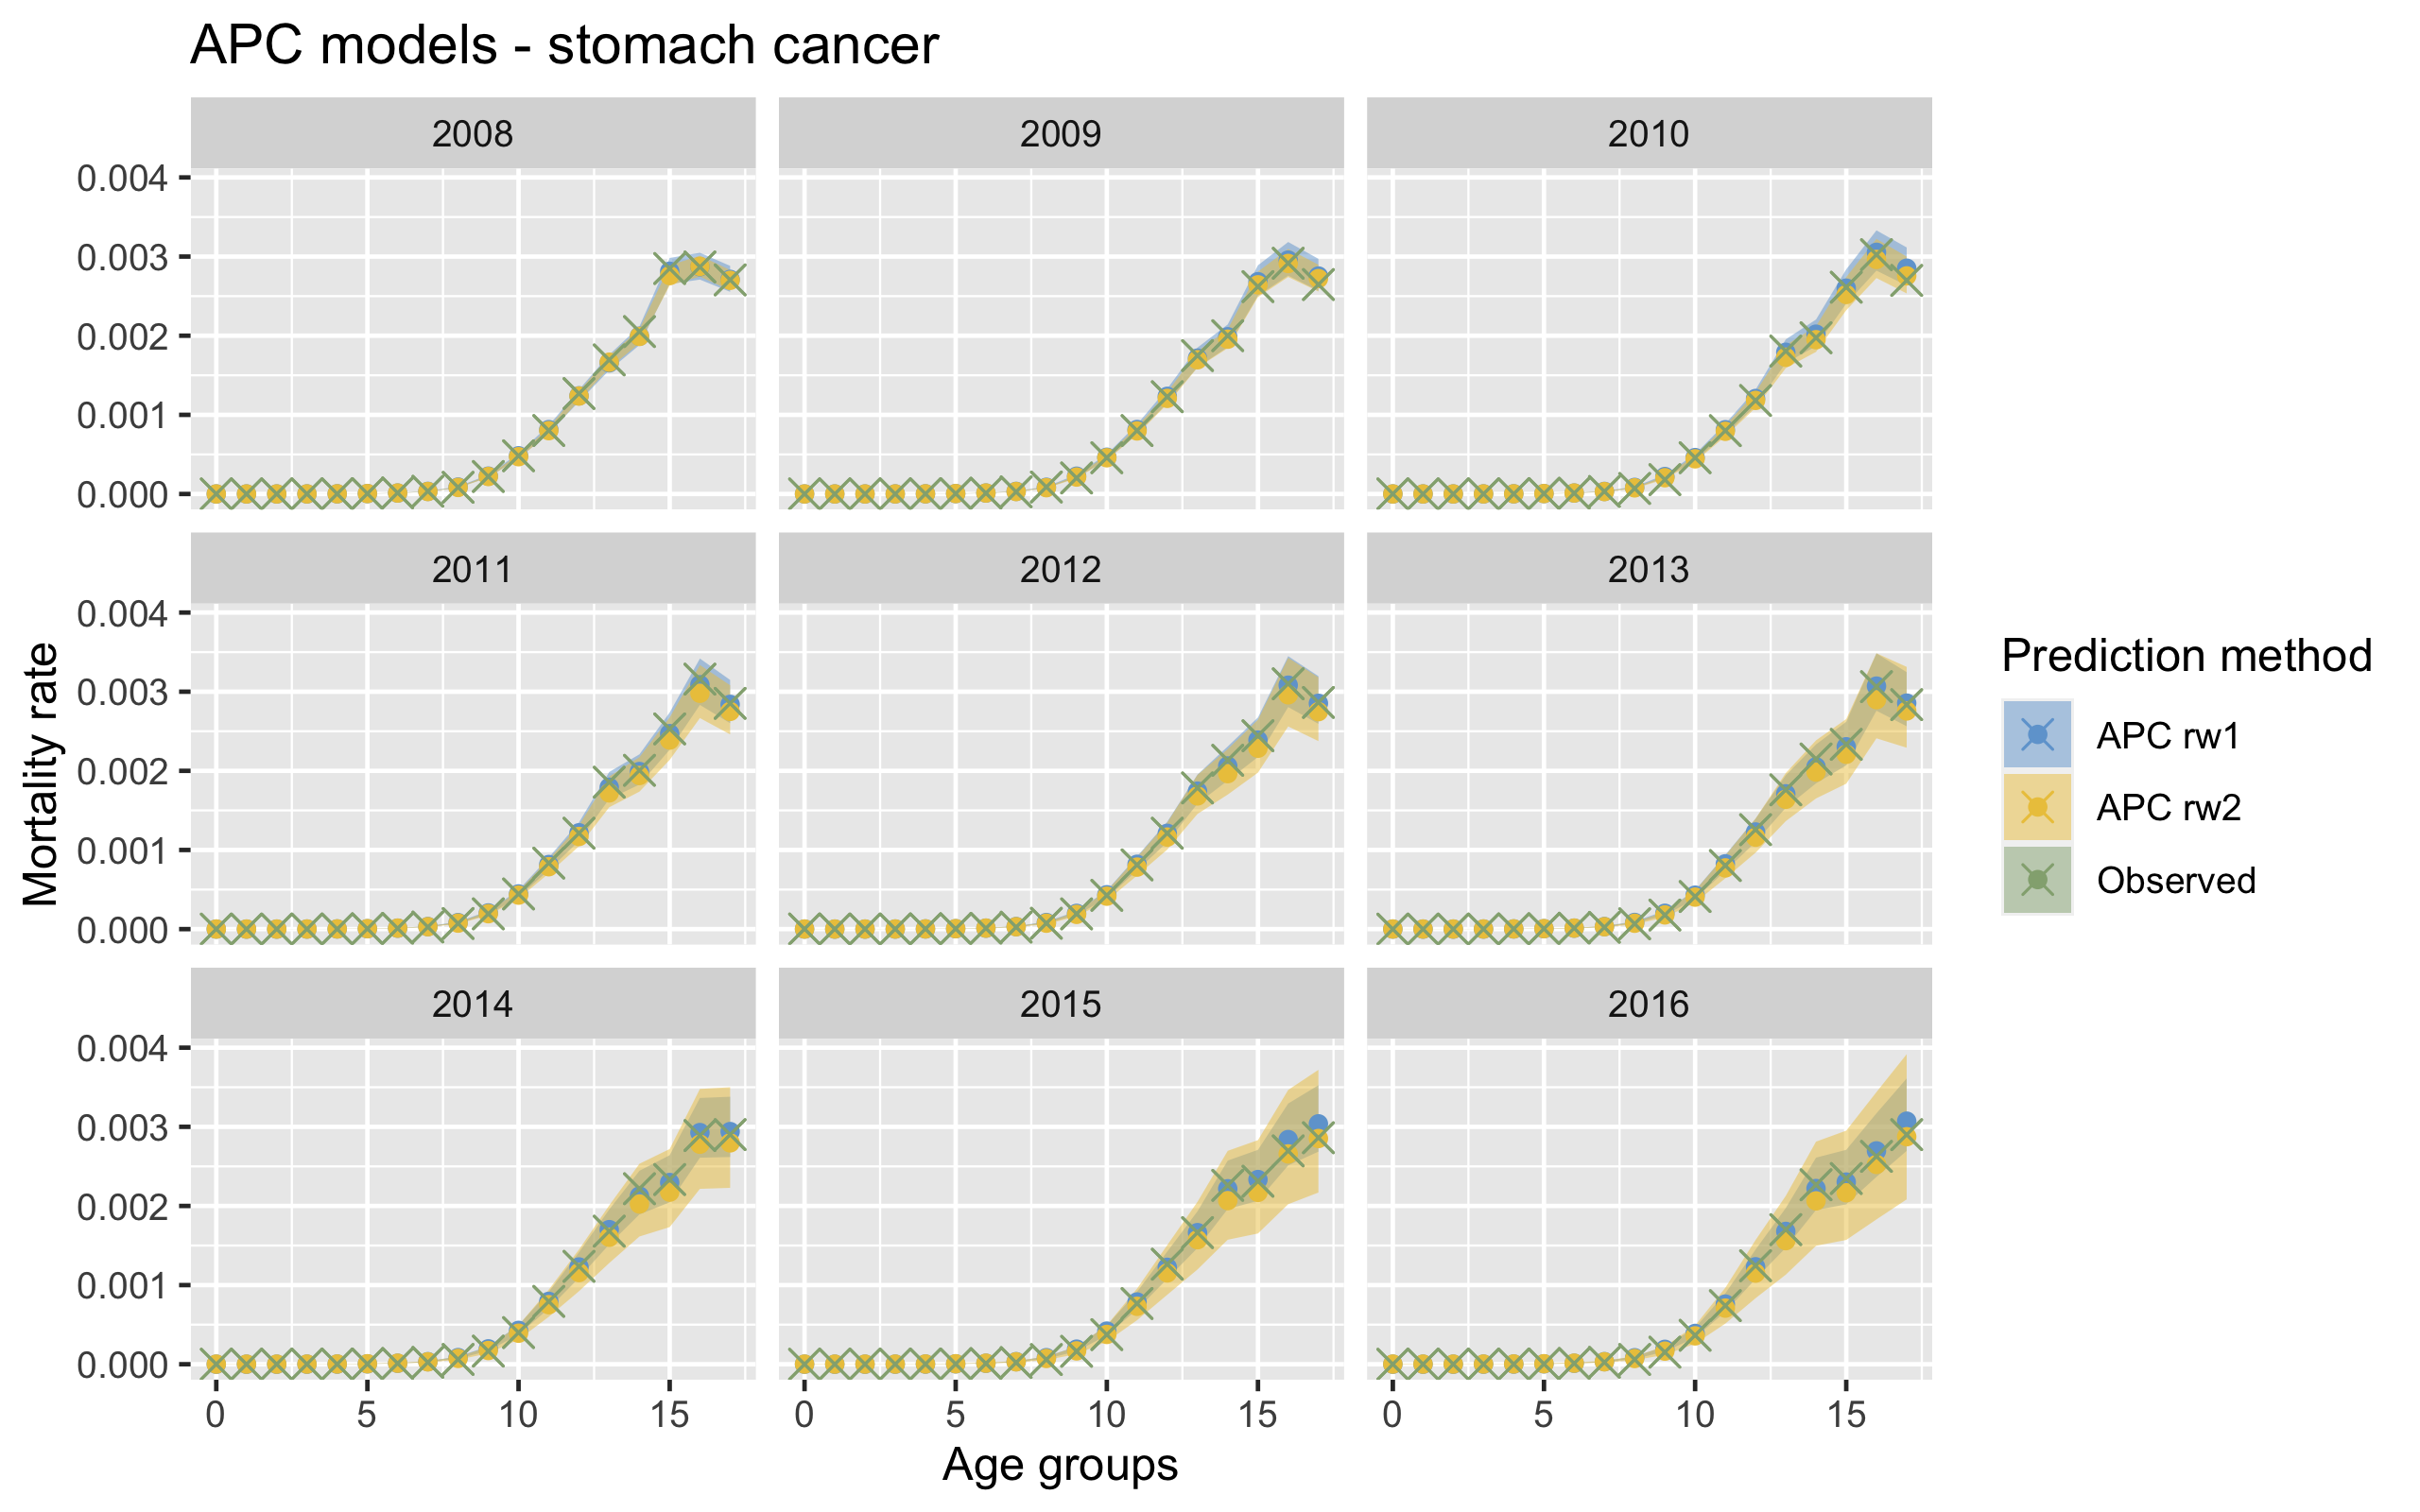
\includegraphics[width=\linewidth]{real-data/real-data-univariate/Figures/univariate-APC-by-age-stomach.png}
        \caption{The prediction results plotted for each of the years that were predicted, with the age groups along the horizontal axis.}
        \label{fig:uv-APC-stomach-top}
    \end{subfigure}
    
    \begin{subfigure}[b]{.75\linewidth}
        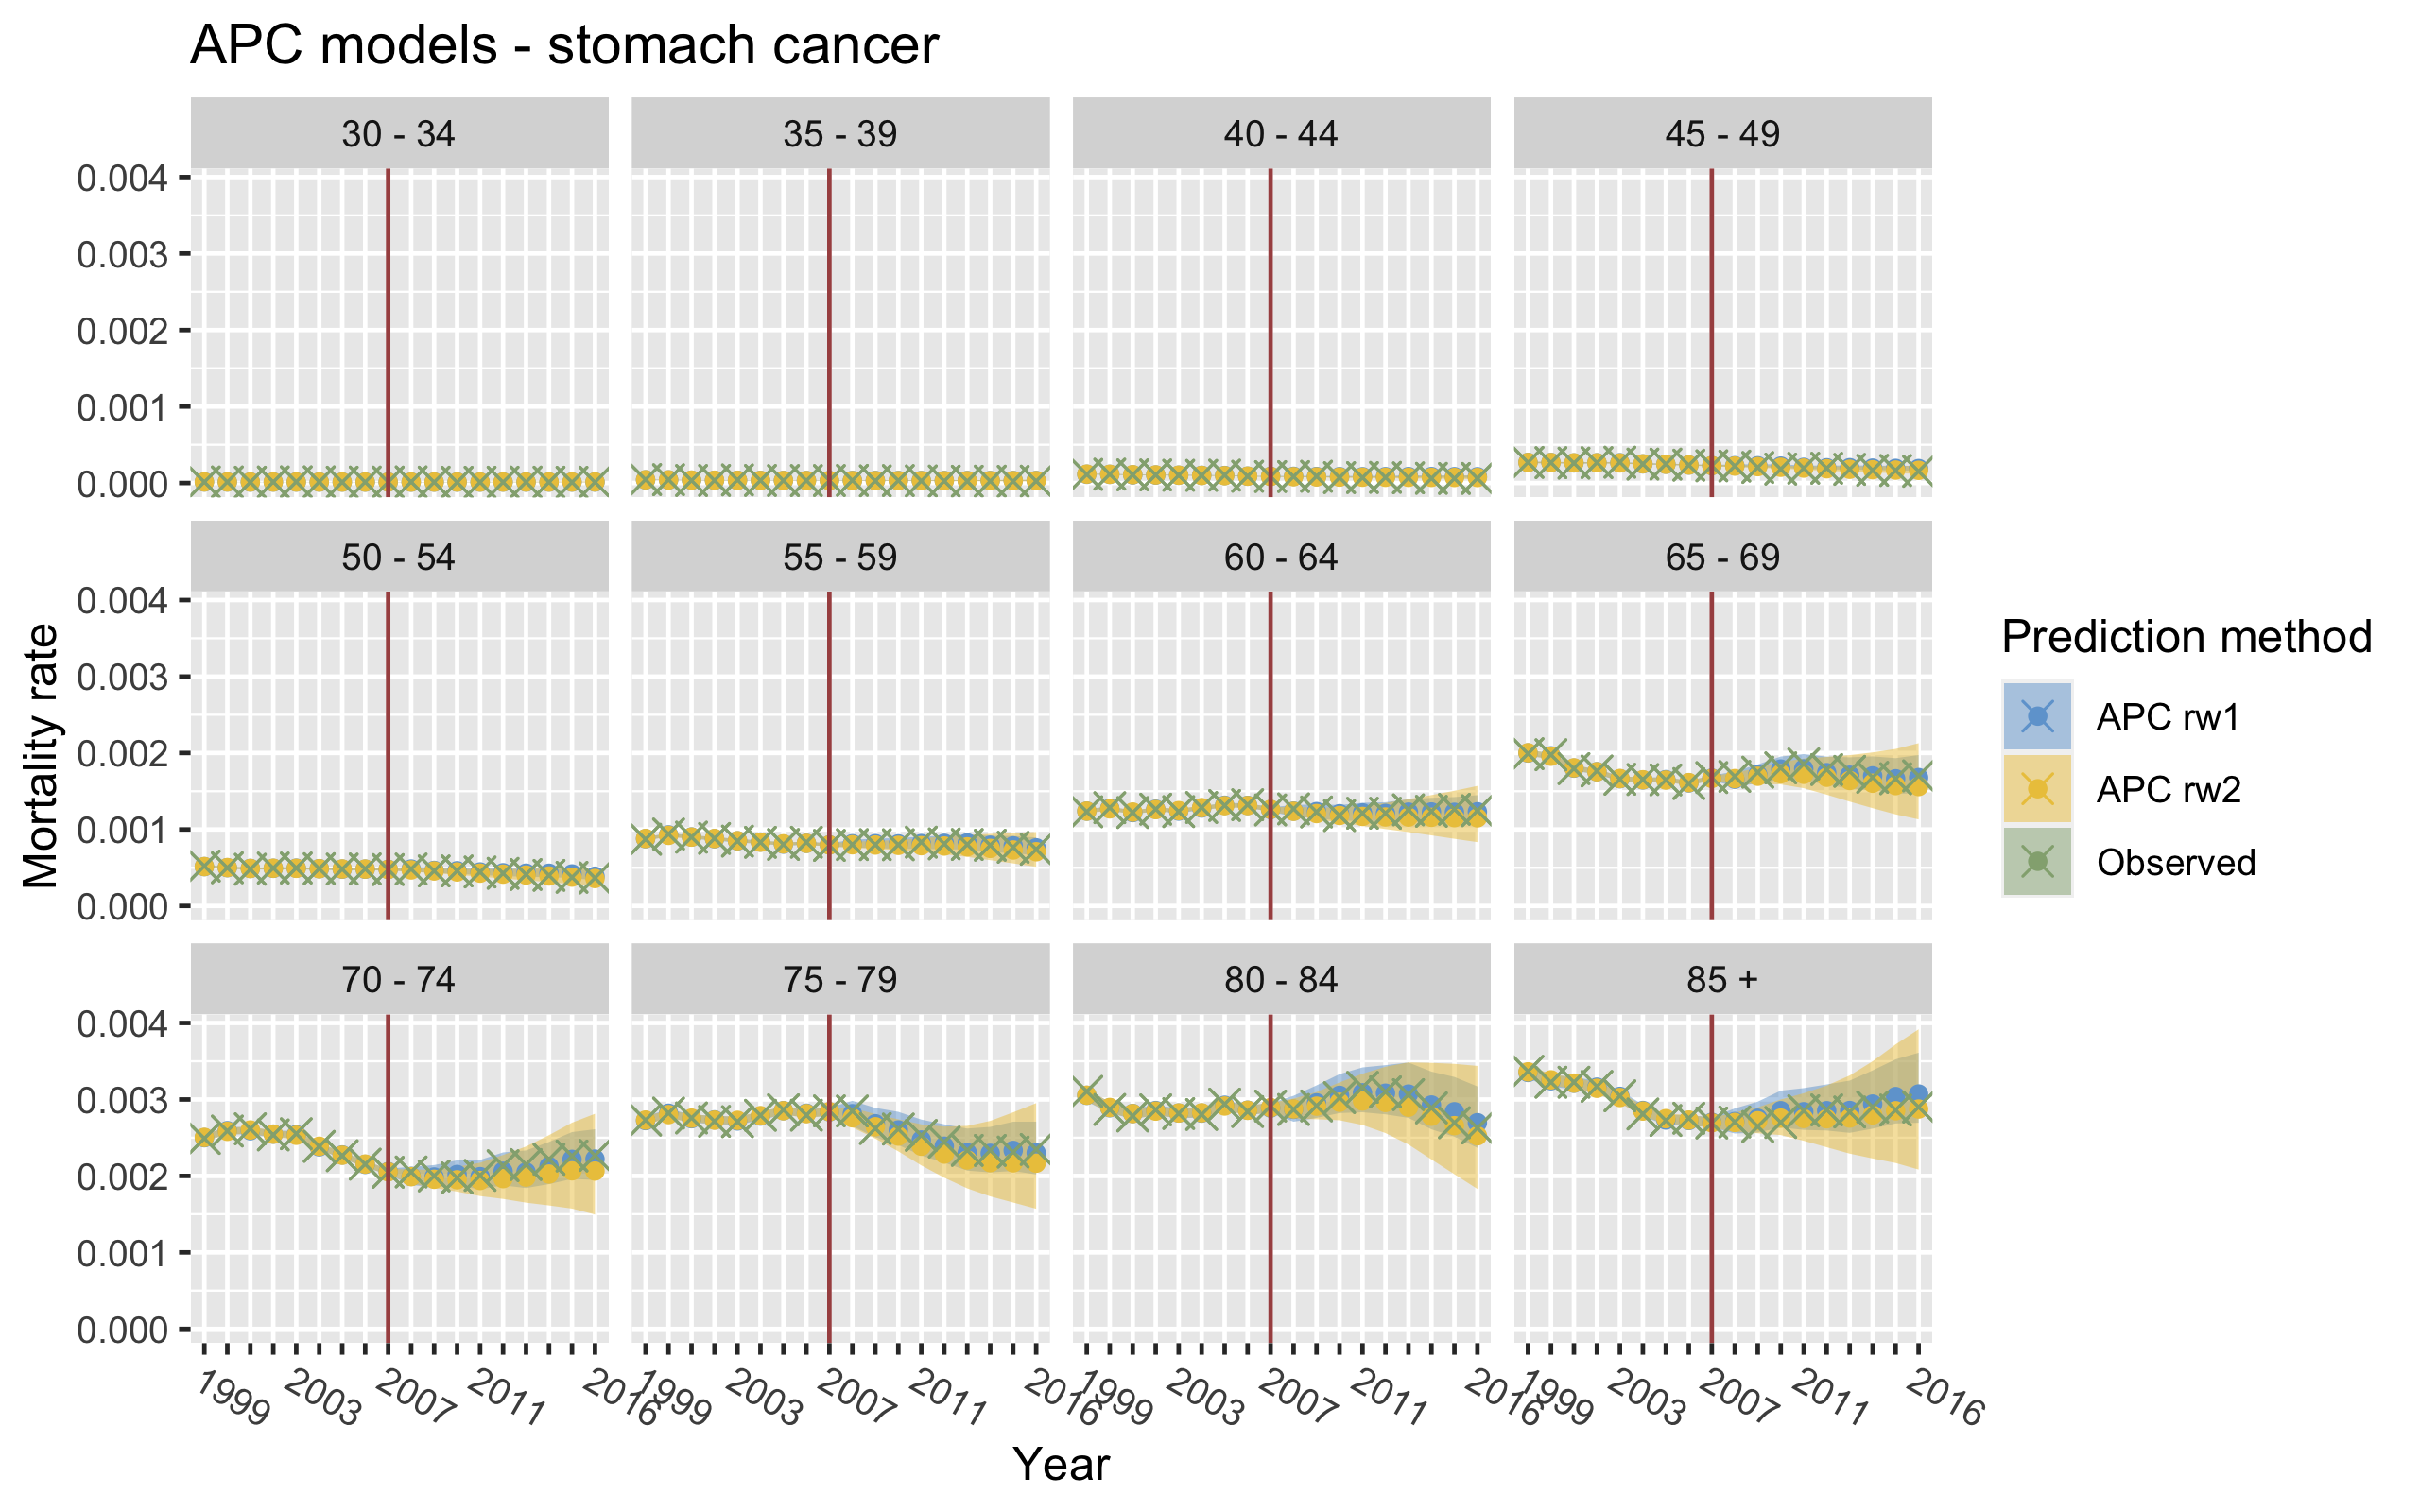
\includegraphics[width=\linewidth]{real-data/real-data-univariate/Figures/univariate-APC-by-period-stomach.png}
        \caption{The prediction results plotted for each age group that are 30 years and older, with the calendar years along the horizontal axis. The red line marks the beginning of the predicted periods.}
        \label{fig:uv-APC-stomach-bottom}
    \end{subfigure}
    \caption{The mean values and the 95\% confidence bounds of the predicted expected stomach cancer mortality rates produced by inference with the APC1- and the APC2-model on data of German stomach cancer (circles), together with the corresponding observed mortality rates $Y_{x,y}^{\text{stomach}}$ (crosses).}
    \label{fig:uv-APC-stomach}
\end{figure}

\begin{table}[h!]
    \begin{center}
        \begin{tabular}{l |c c c }
            Model & MSE &   MDSS & Contained 95\%-interval\\
            \hline
            APC1    & 2.591e-9 & -18.63    & 0.9383 \\
            APC2    & 7.774e-9 & -18.35    & 0.9877 \\
            LC         & 9.134e-8 & -12.60    & 0.4938 \\
            LCC        & 1.481e-8 & -17.99    & 0.9383 \\ 
            LCC-linear & 1.520e-8 & -17.89    & 0.8889 \\
        \end{tabular}
        \caption{Score statistics for different models applied to the stomach cancer data, calculated for predictions where $x > 8$.}\label{tbl:uv-stomach-8}
    \end{center}
\end{table}

\begin{figure}[h!]
    \centering
    \begin{subfigure}[b]{.75\linewidth}
        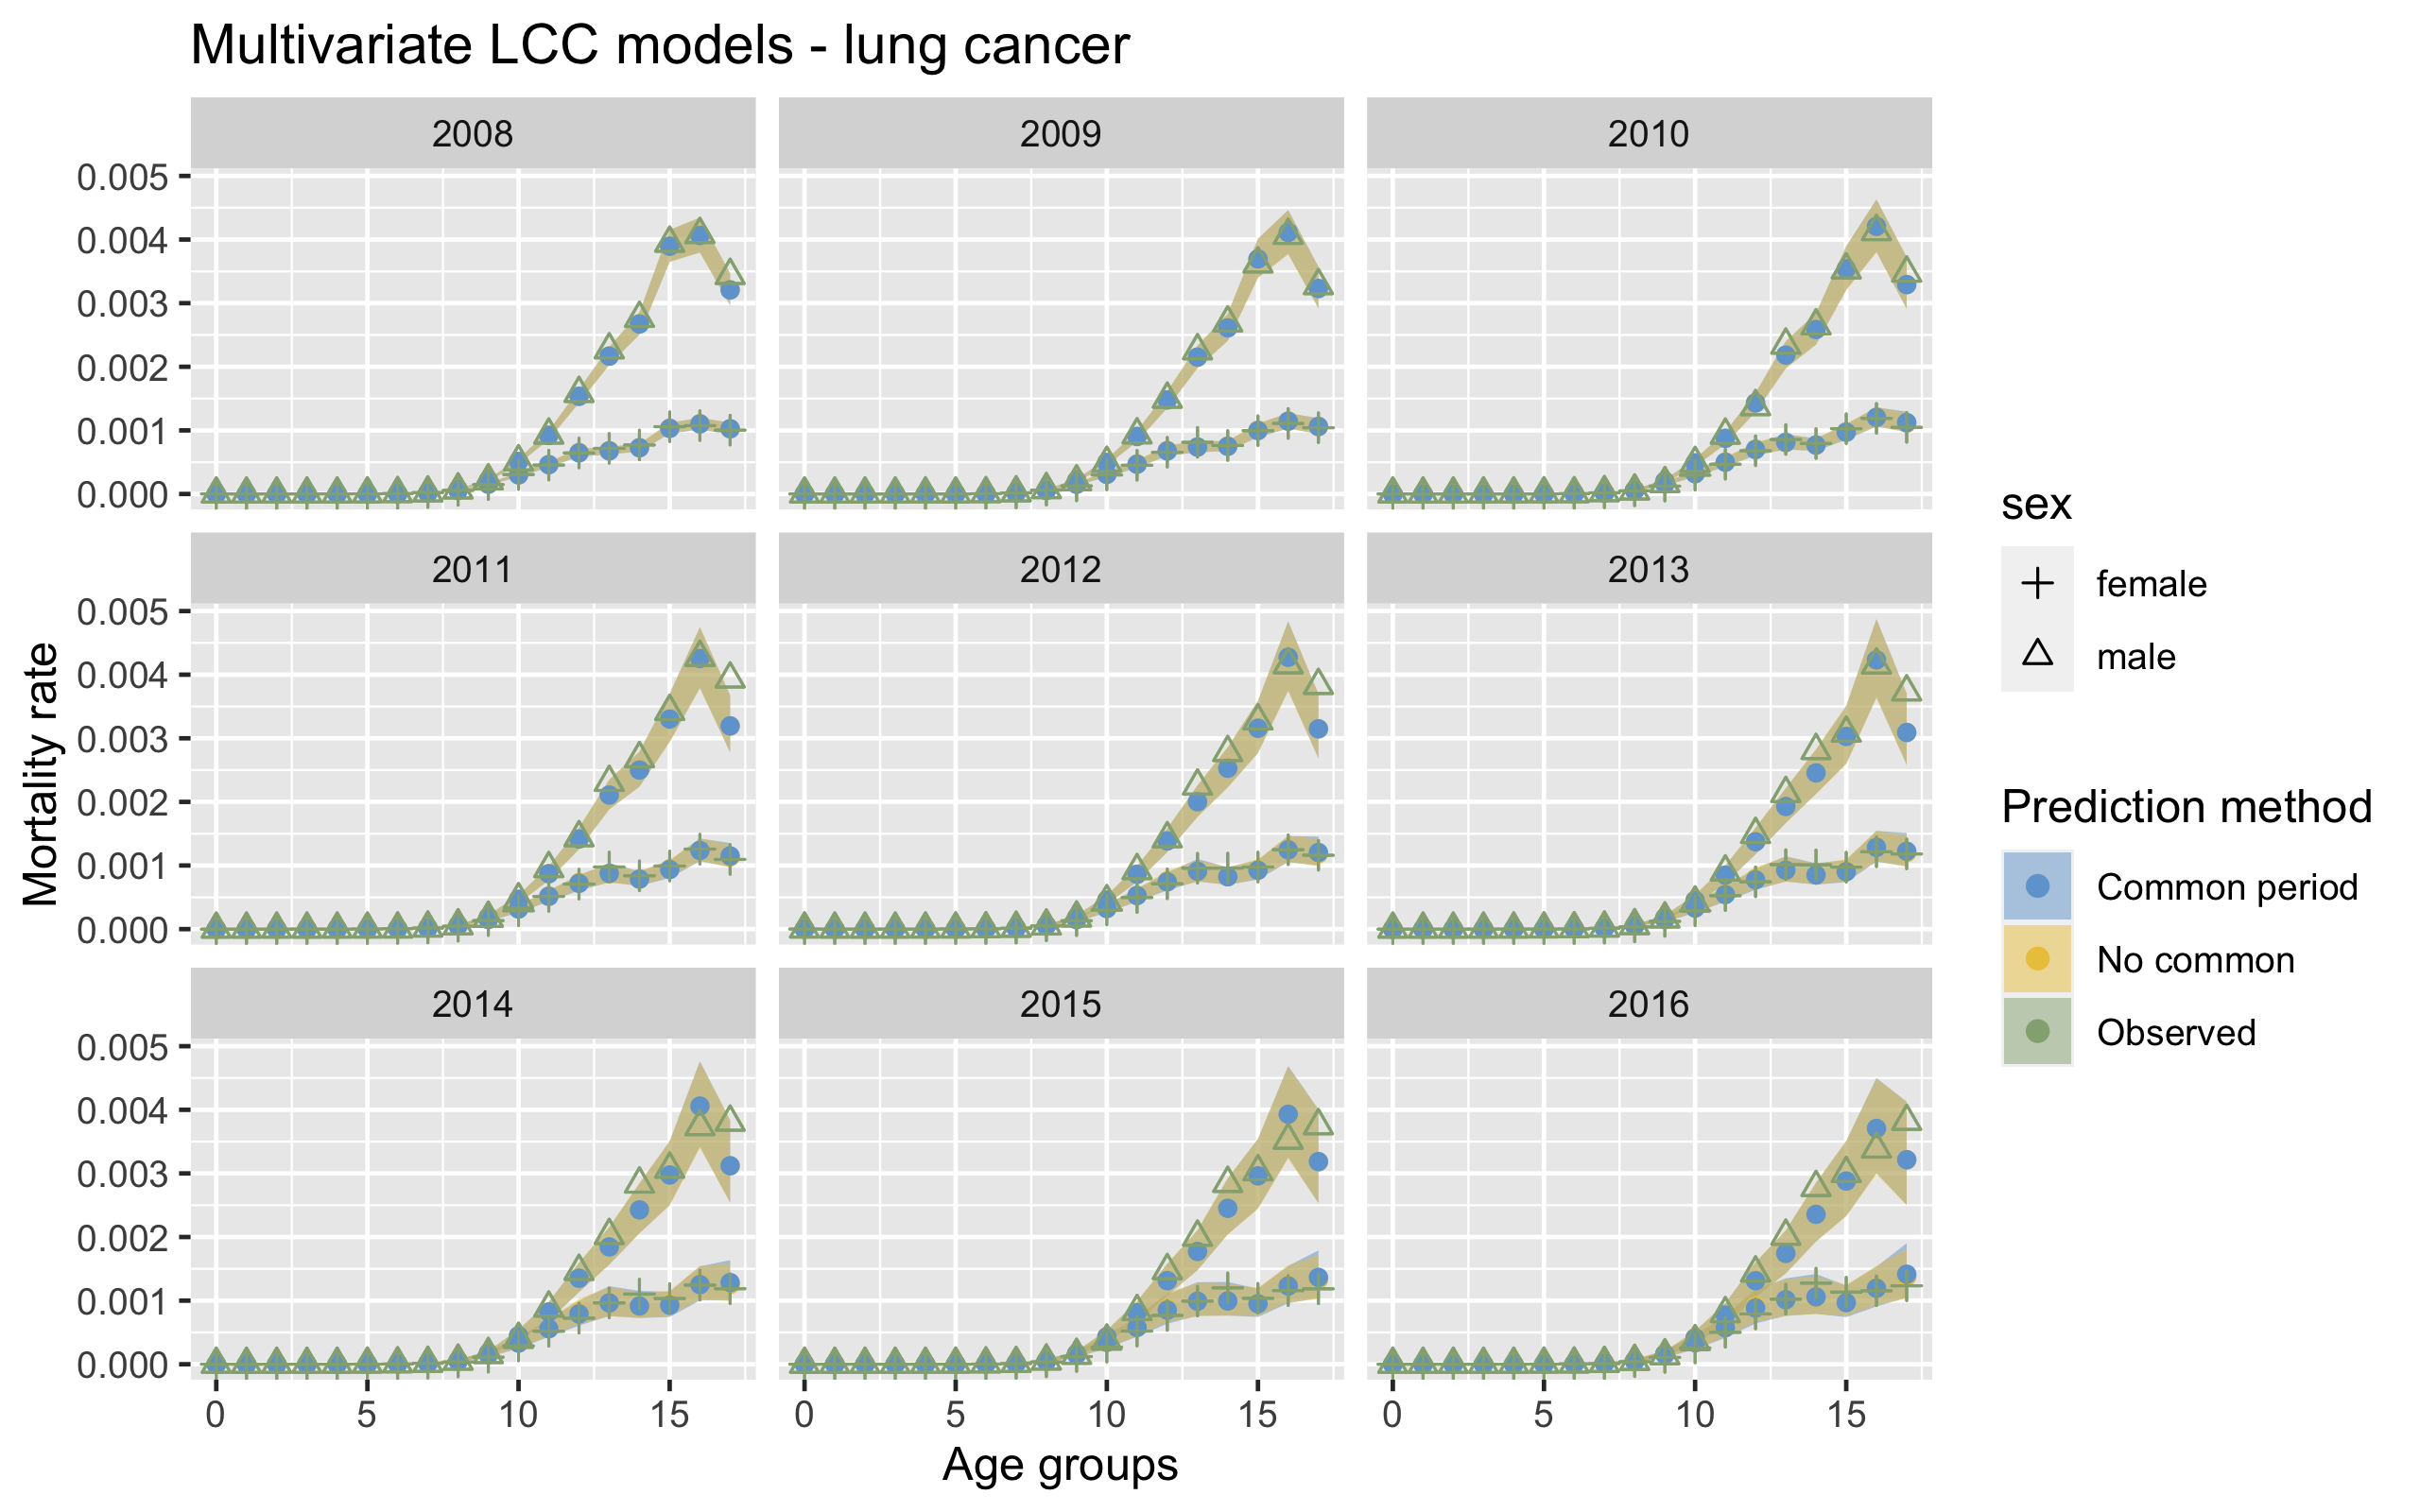
\includegraphics[width=\linewidth]{real-data/real-data-multivariate/Figures/multivariate-LCC-by-age-lung.png}
        \caption{The prediction results plotted for each of the years that were predicted, with the age groups along the horizontal axis.}
        \label{fig:mv-LCC-lung-top}
    \end{subfigure}
    
    \begin{subfigure}[b]{.75\linewidth}
        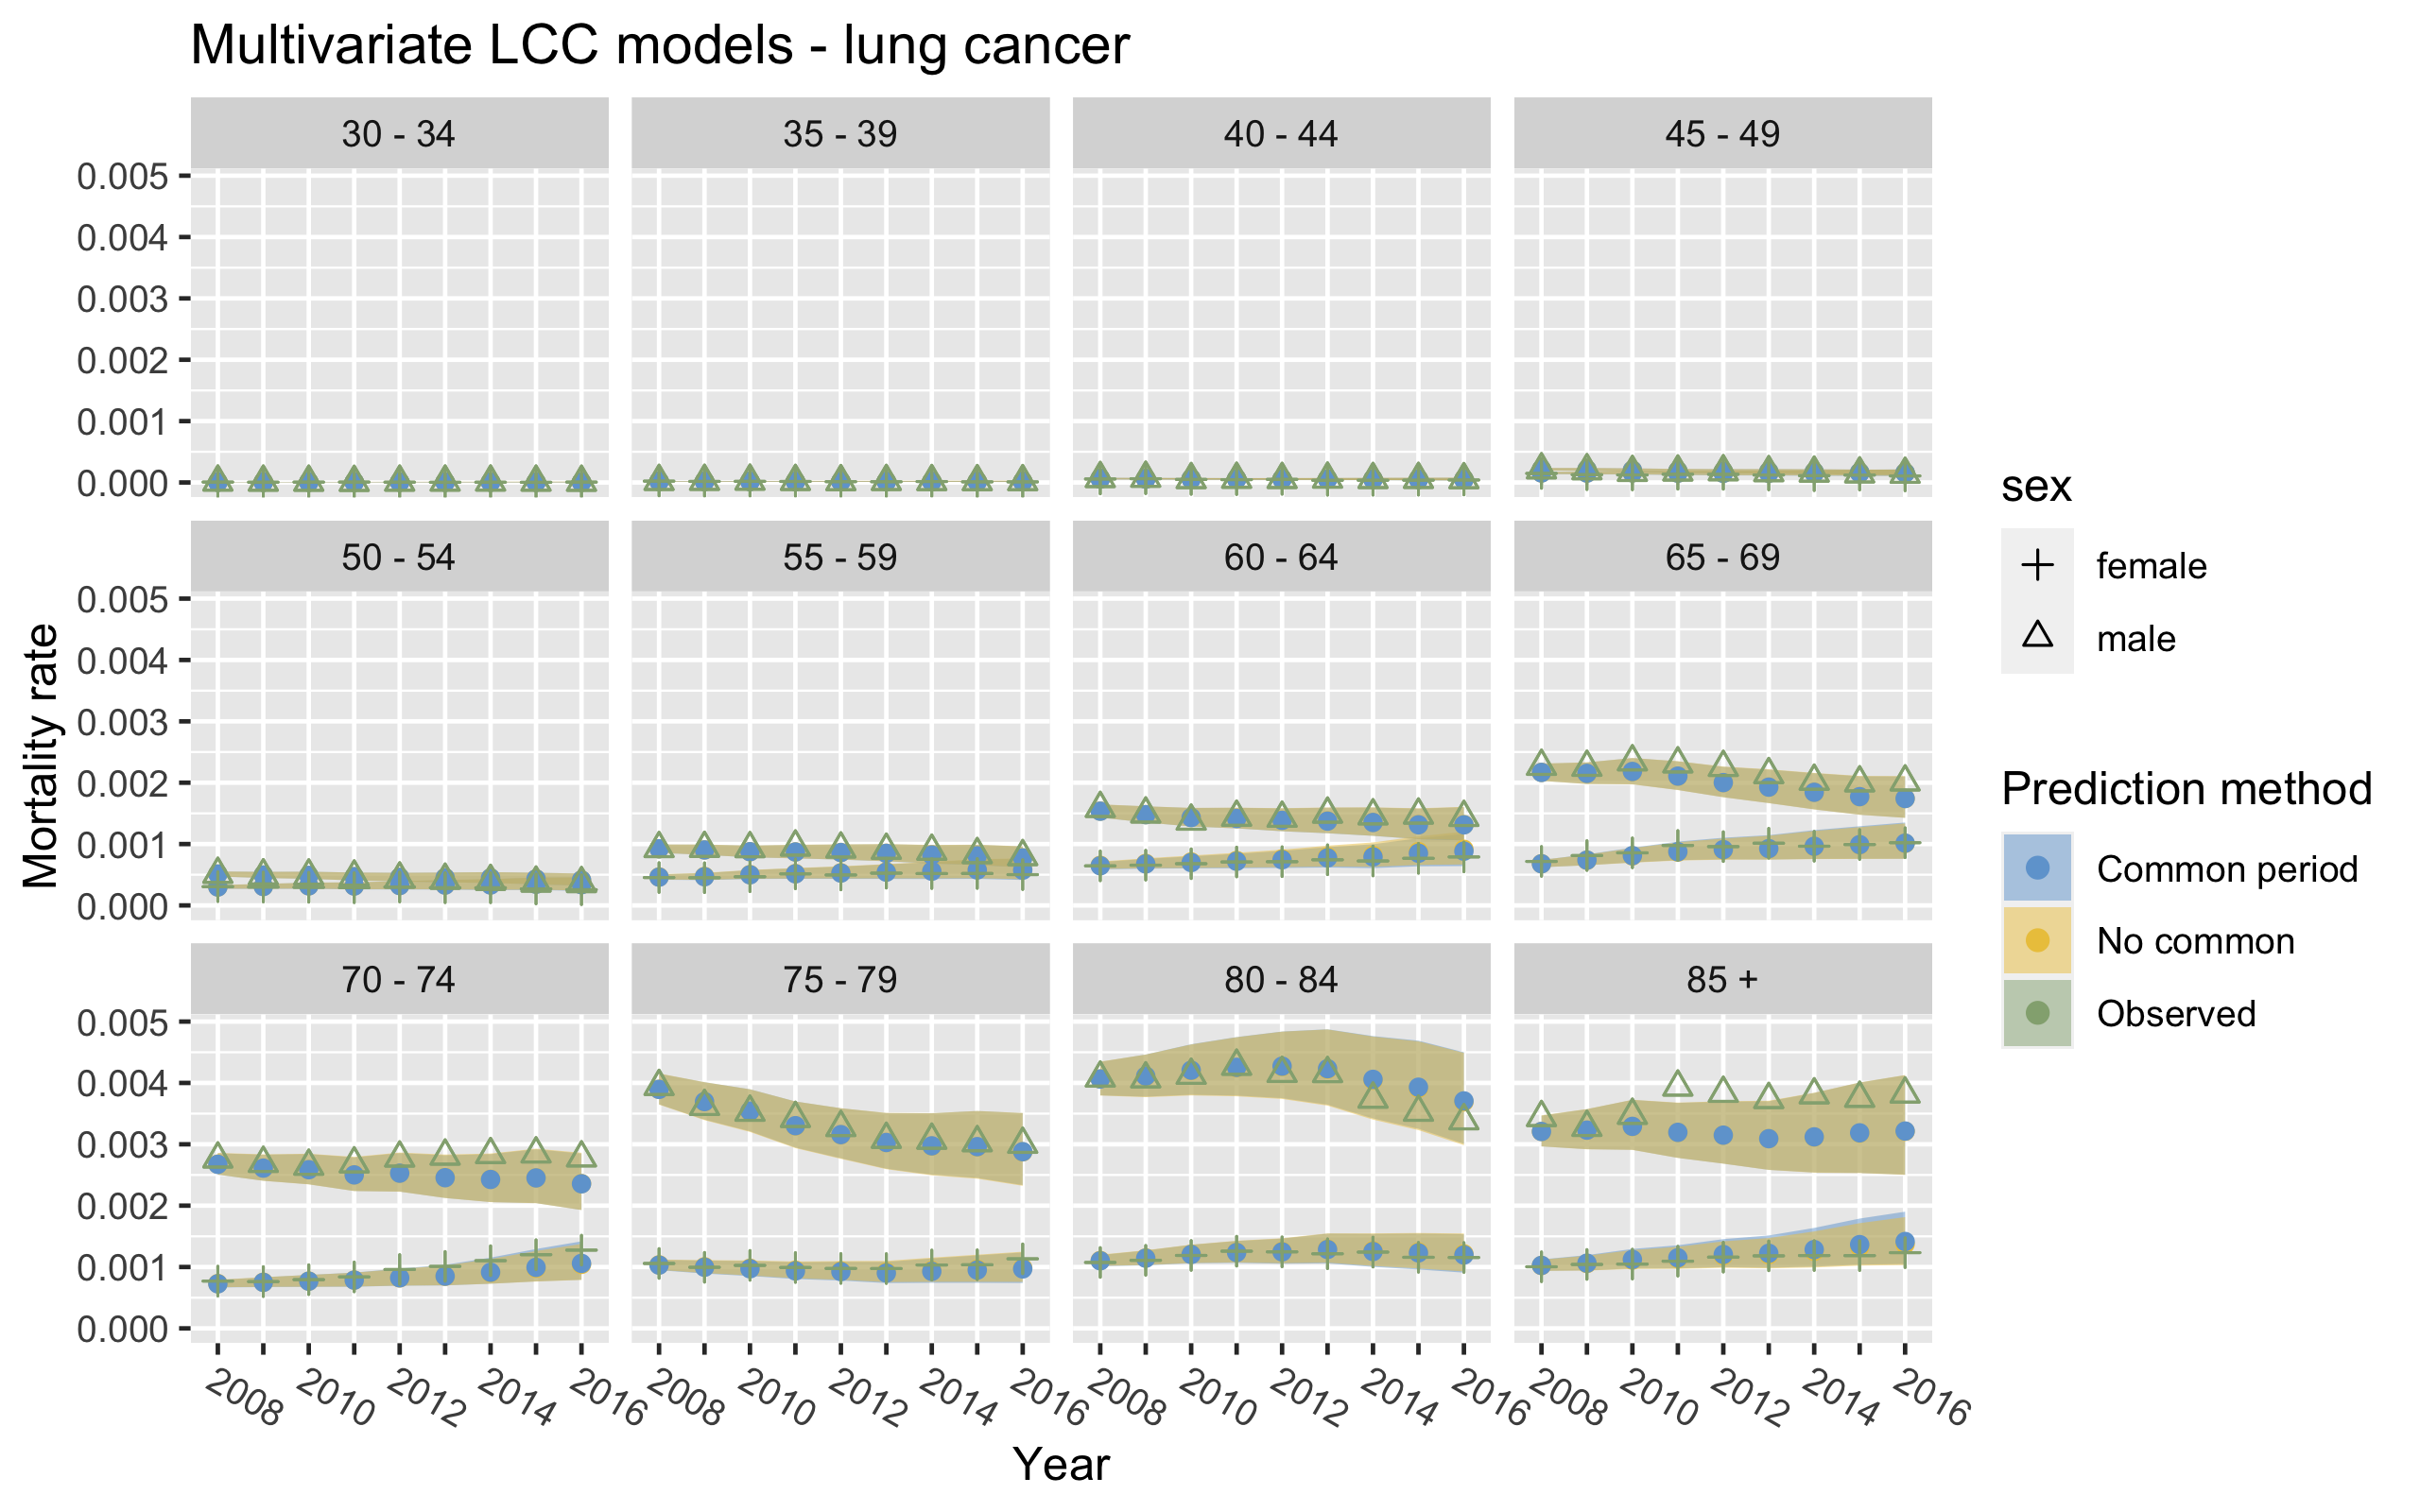
\includegraphics[width=\linewidth]{real-data/real-data-multivariate/Figures/multivariate-LCC-by-period-lung.png}
        \caption{The prediction results plotted for each age group that are 30 years and older, with the calendar years along the horizontal axis. The red line marks the beginning of the predicted periods.}
        \label{fig:mv-LCC-lung-bottom}
    \end{subfigure}
    
    \caption{The mean values and the 95\% confidence bounds of the predicted expected lung cancer mortality rates produced by inference with the "Common period"-model and the "No common"-model on data of German lung cancer (circles), together with the corresponding observed male mortality rates $Y_{x,y}^{\text{lung, male}}$ (triangles) and female mortality rates $Y_{x,y}^{\text{lung, female}}$ (crosses).}
    \label{fig:mv-LCC-lung}
\end{figure}

\begin{figure}[h!]
    \centering
    \begin{subfigure}[b]{.75\linewidth}
        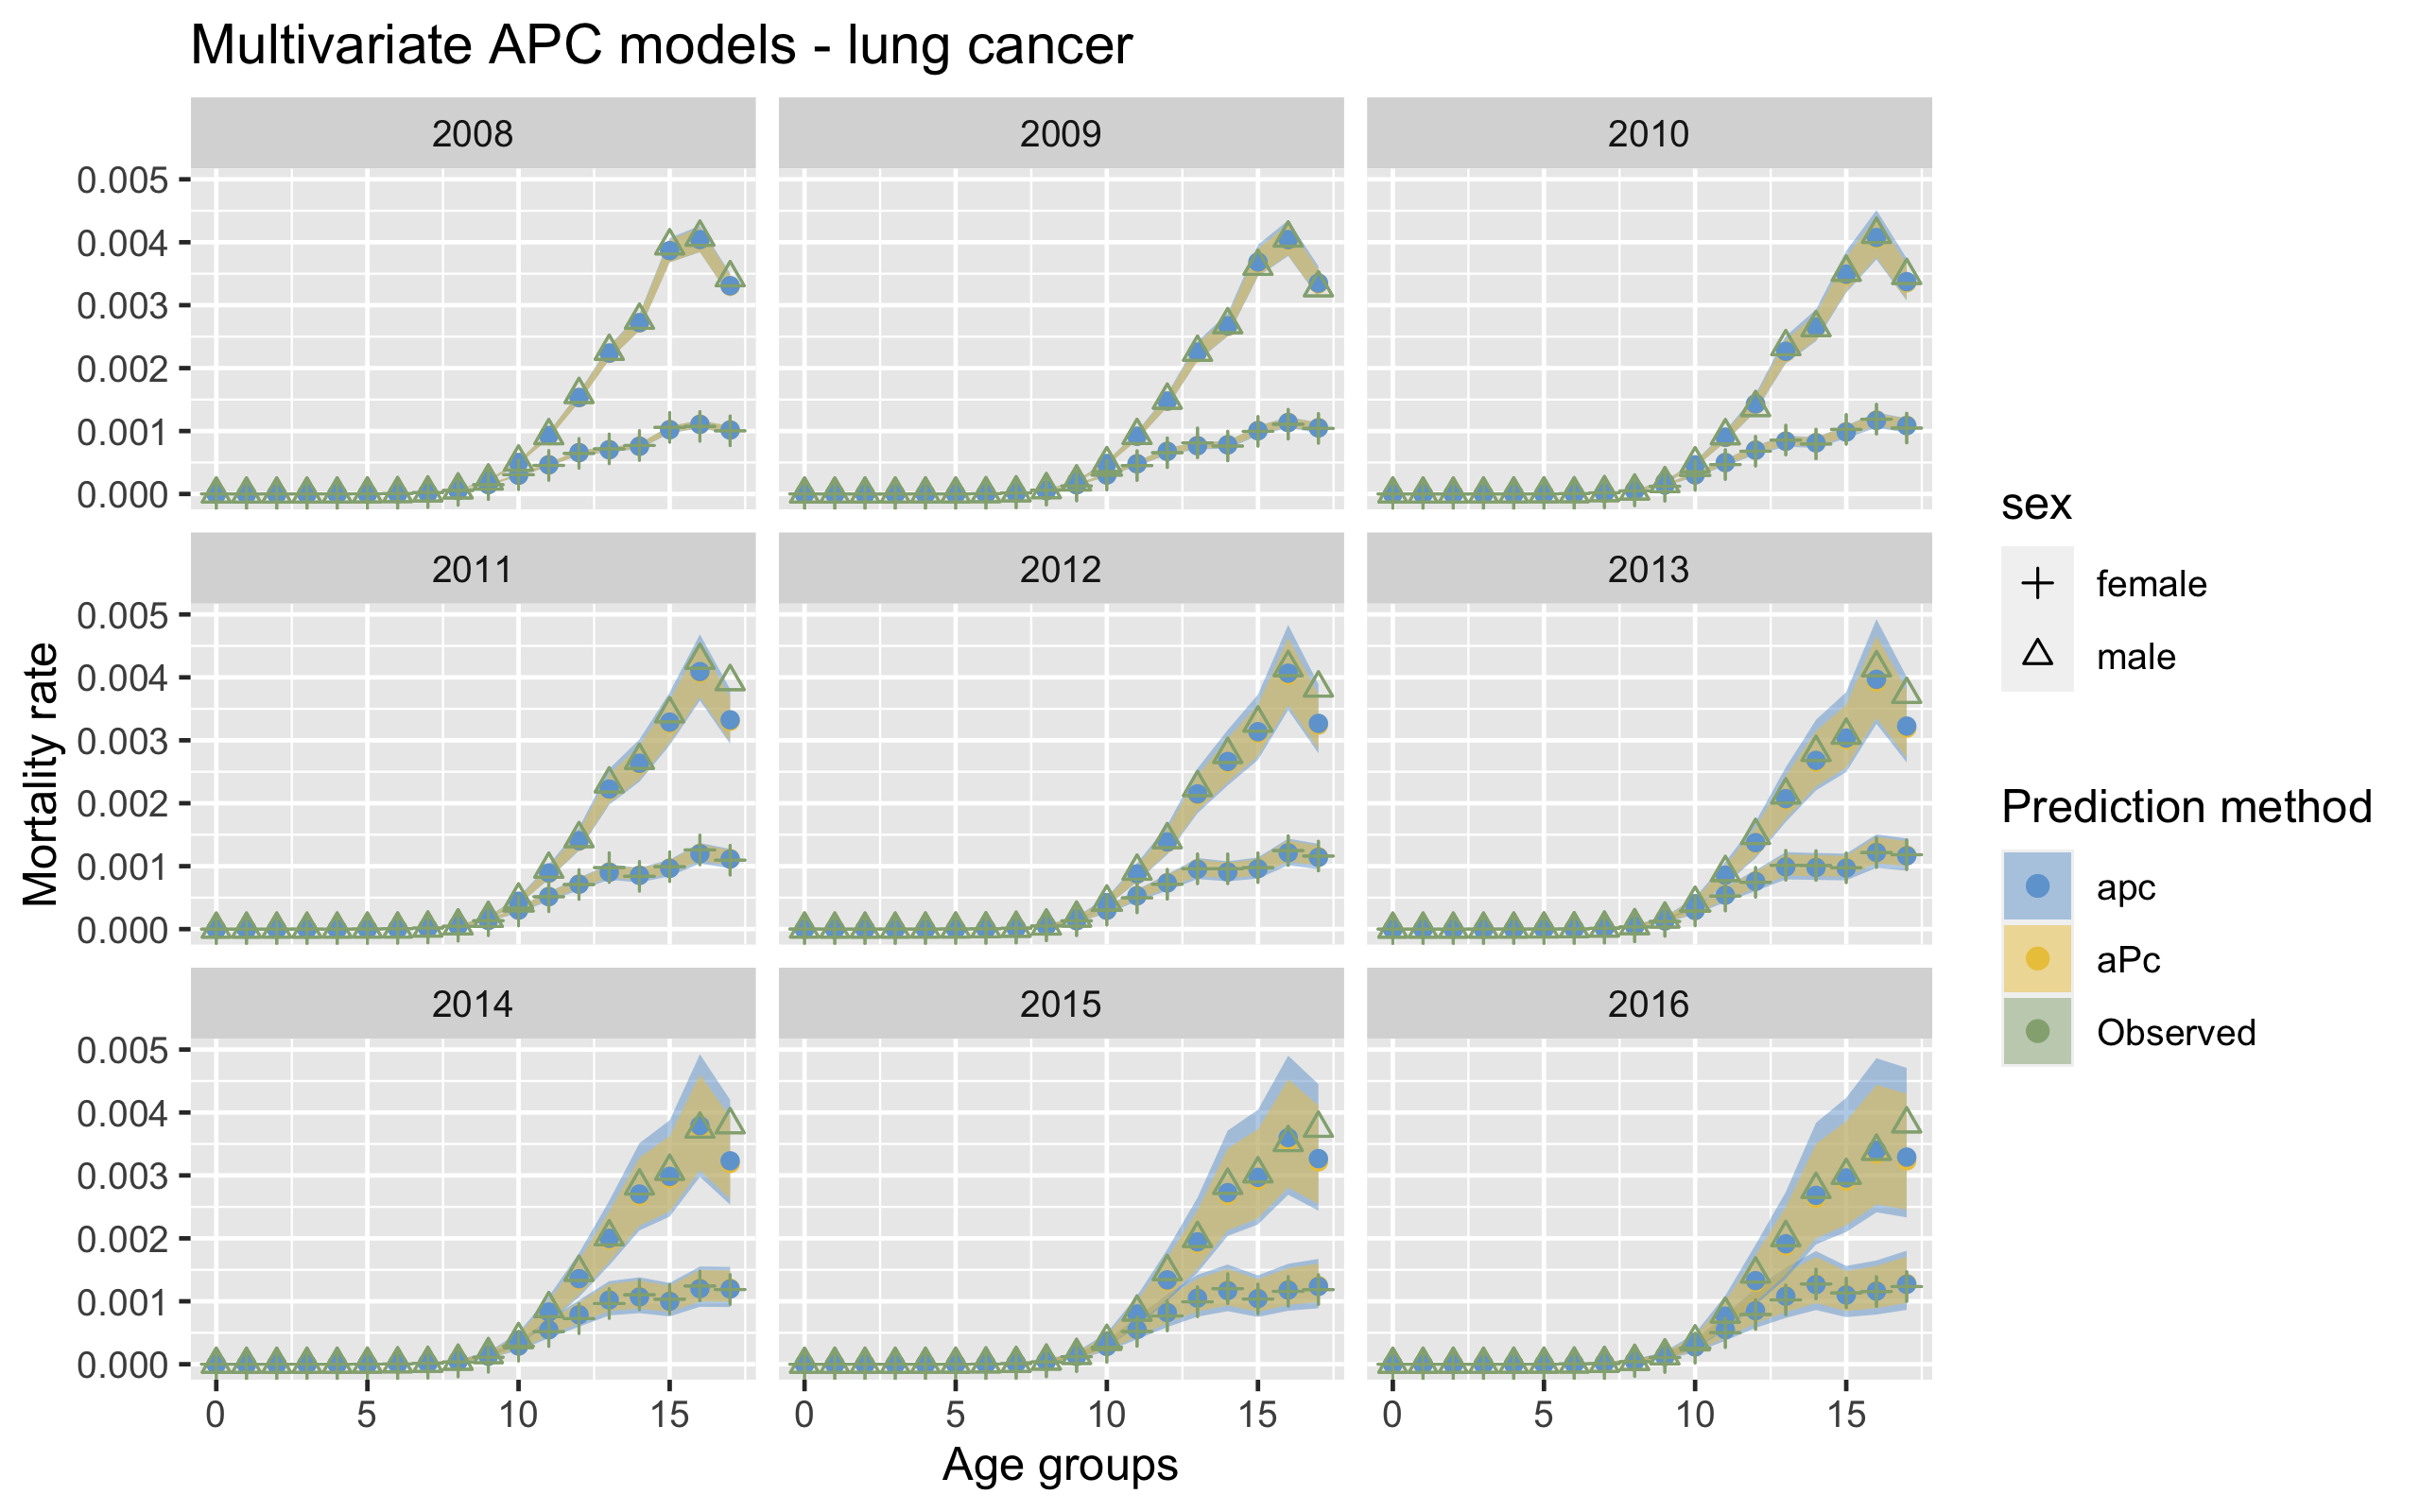
\includegraphics[width=\linewidth]{real-data/real-data-multivariate/Figures/multivariate-APC-by-age-lung.png}
        \caption{The prediction results plotted for each of the years that were predicted, with the age groups along the horizontal axis.}
        \label{fig:mv-APC-lung-top}
    \end{subfigure}
    
    \begin{subfigure}[b]{.75\linewidth}
        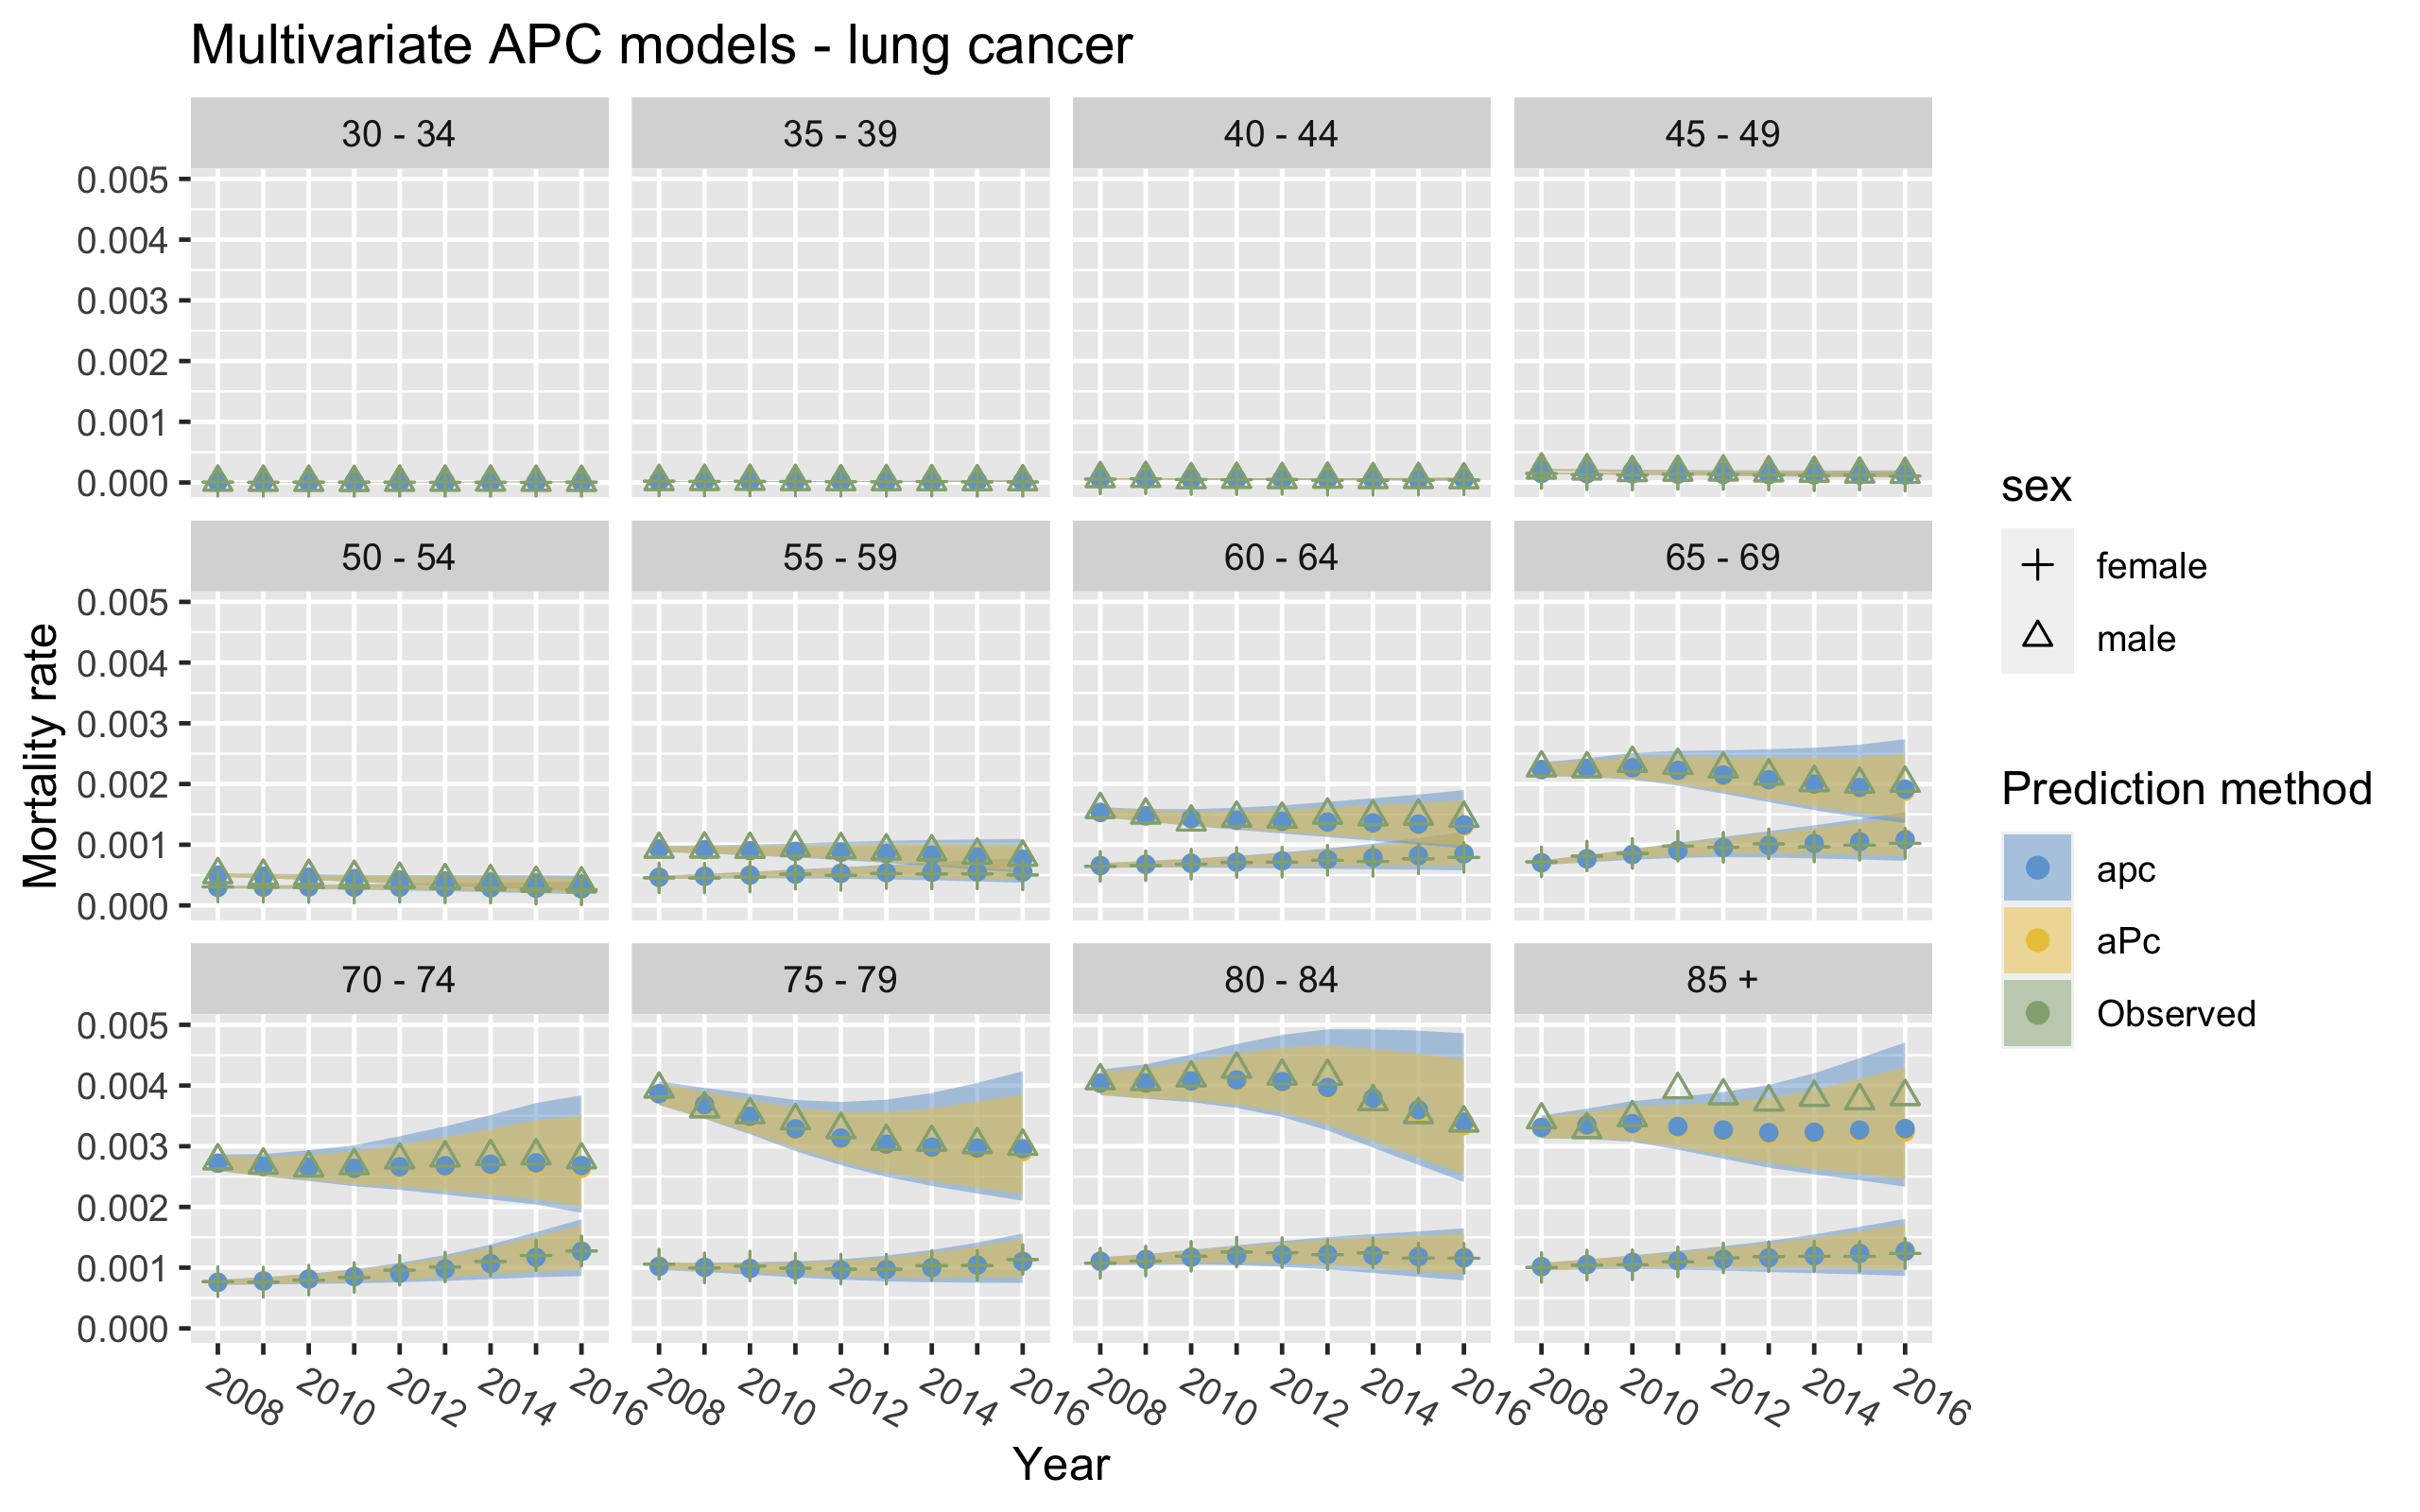
\includegraphics[width=\linewidth]{real-data/real-data-multivariate/Figures/multivariate-APC-by-period-lung.png}
        \caption{The prediction results plotted for each age group that are 30 years and older, with the calendar years along the horizontal axis. The red line marks the beginning of the predicted periods.}
        \label{fig:mv-APC-lung-bottom}
    \end{subfigure}
    
    \caption{The mean values and the 95\% confidence bounds of the predicted expected lung cancer mortality rates produced by inference with the apc-model and the aPc-model on data of German lung cancer (circles), together with the corresponding observed male mortality rates $Y_{x,y}^{\text{lung, male}}$ (triangles) and female mortality rates $Y_{x,y}^{\text{lung, female}}$ (crosses).}
    \label{fig:mv-APC-lung}
\end{figure}

\begin{figure}[h!]
    \centering
    \begin{subfigure}[b]{.75\linewidth}
        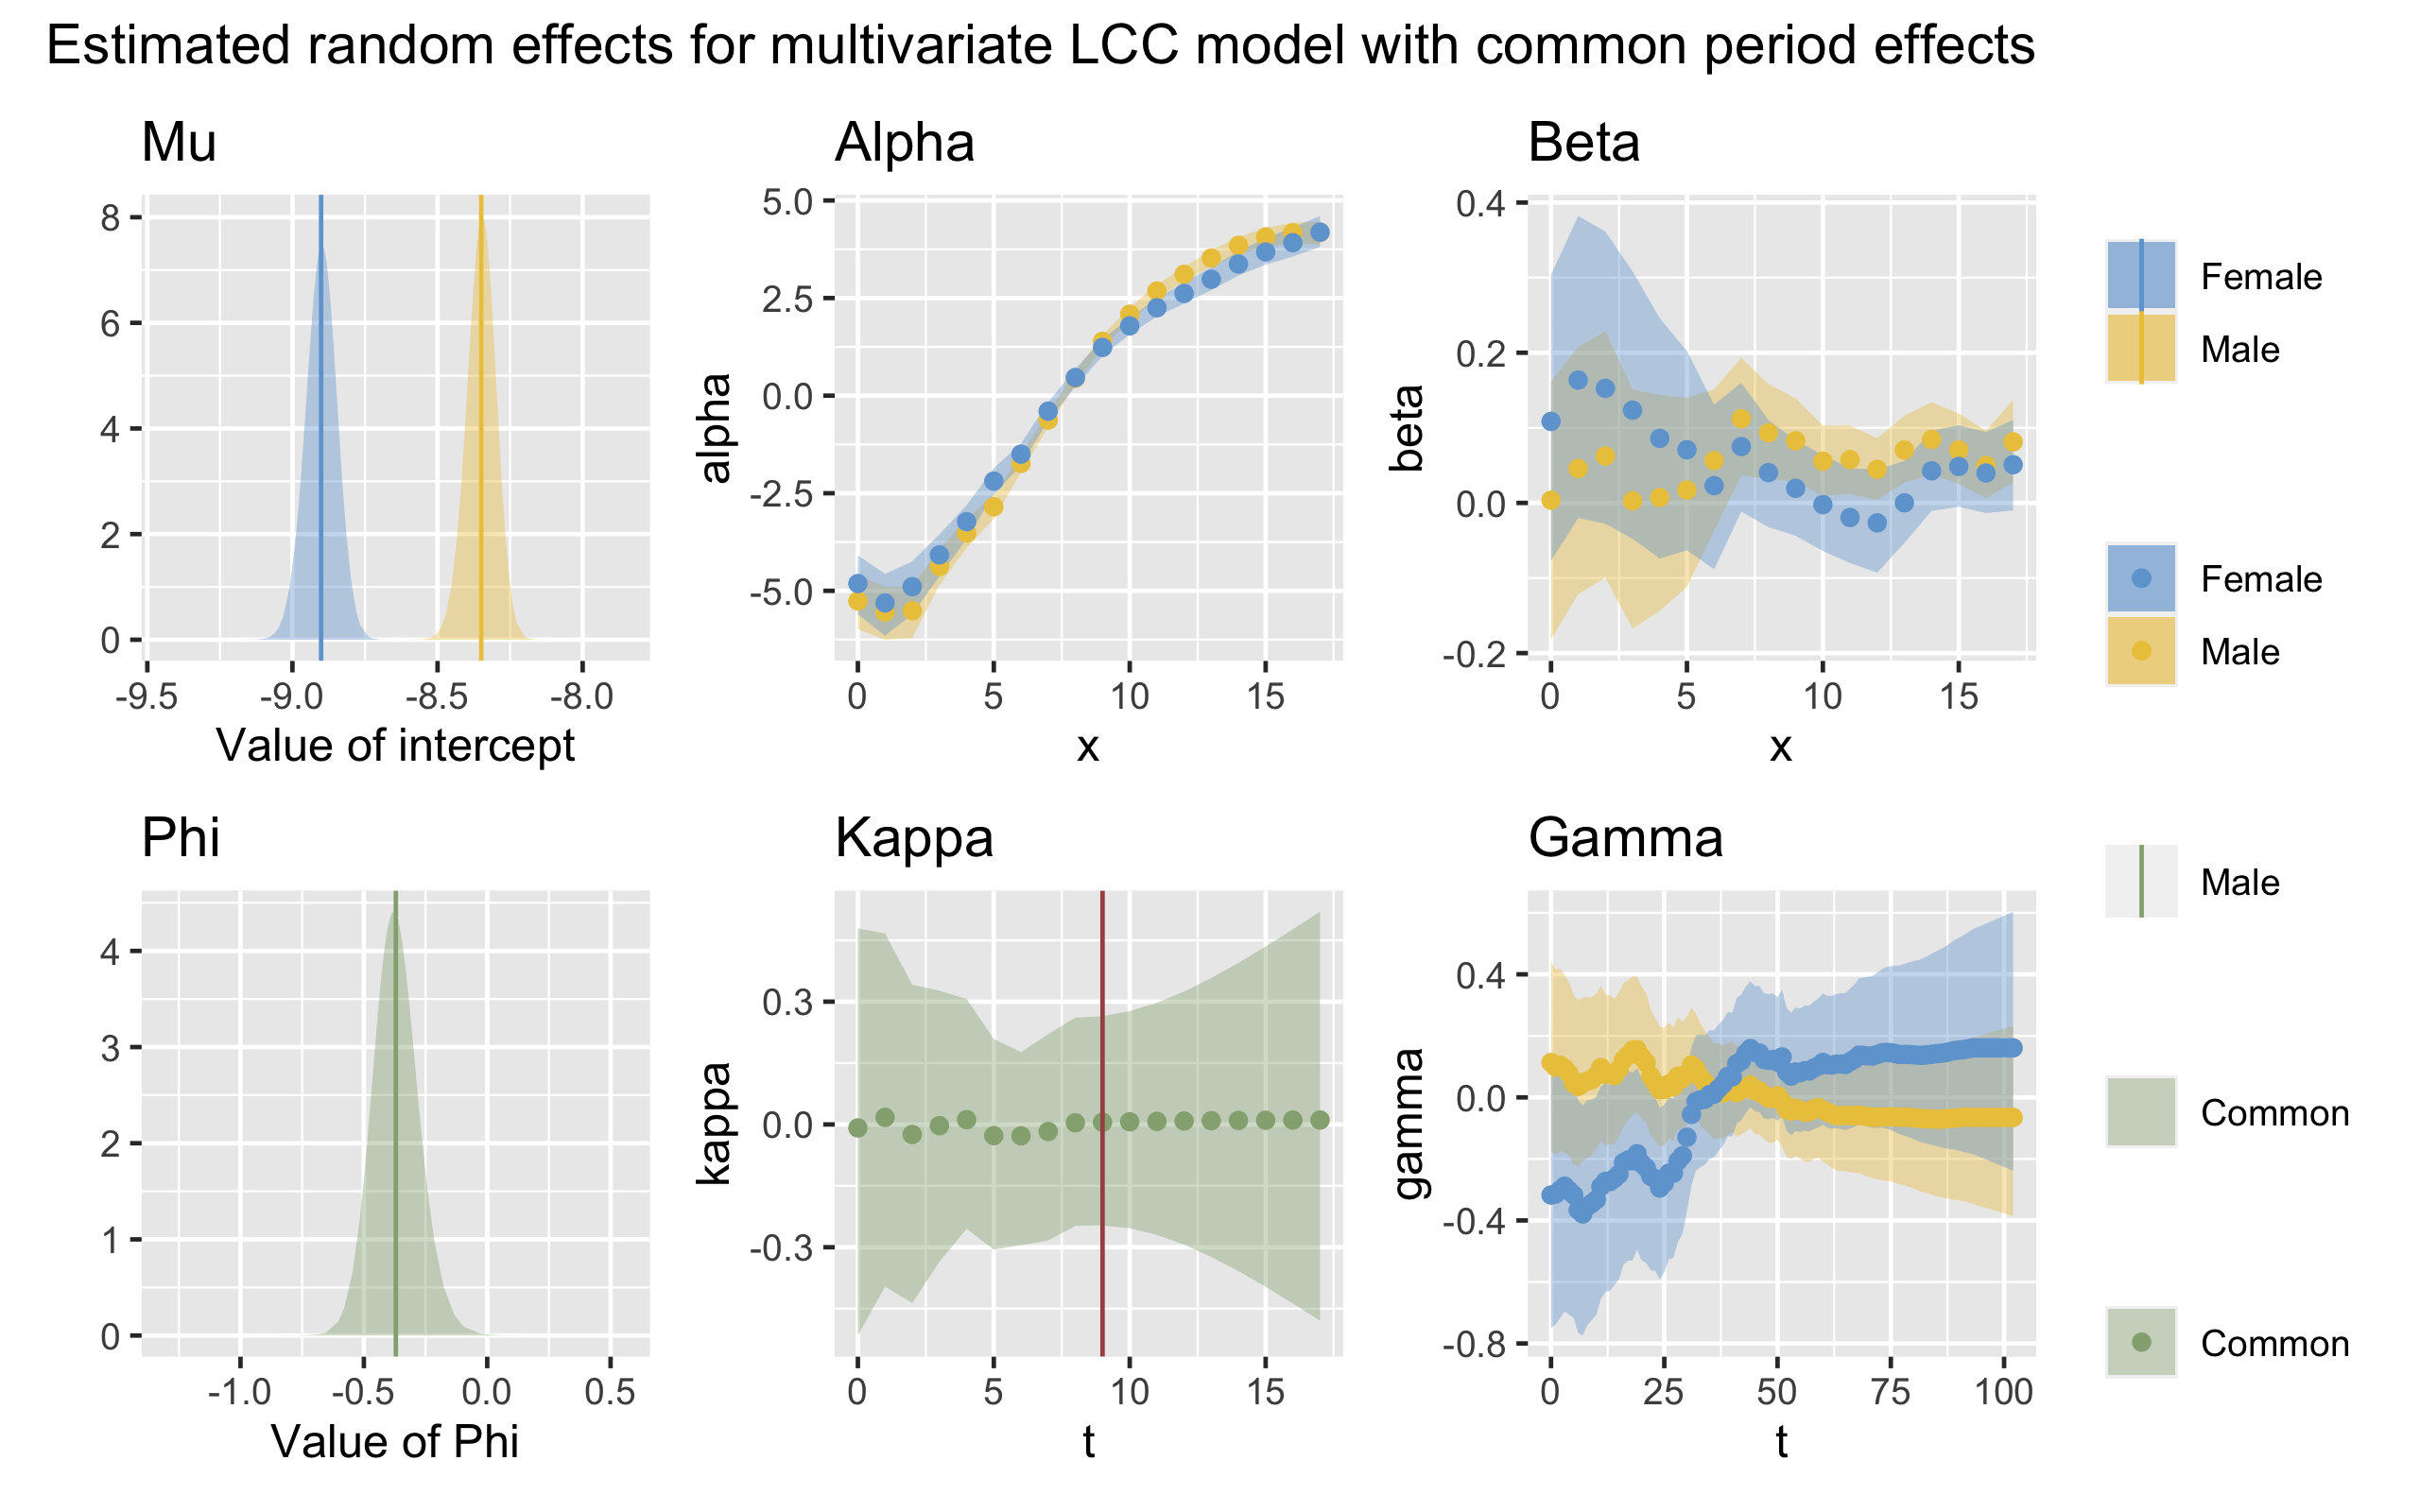
\includegraphics[width=\linewidth]{real-data/real-data-multivariate/Figures/effects-LCC-common-period-stomach.png}
        \caption{The estimated overall mortality level $\mu^{\text{sex}}$ and the estimated random effects $\alpha_x^{\text{sex}}$, $\beta_x^{\text{sex}}$, $\phi$, $\kappa_t$ and $\gamma_k^{\text{sex}}$ produced with inference with the "Common period"-model.}
        \label{fig:effects-LCC-stomach-top}
    \end{subfigure}
    
    \begin{subfigure}[b]{.75\linewidth}
        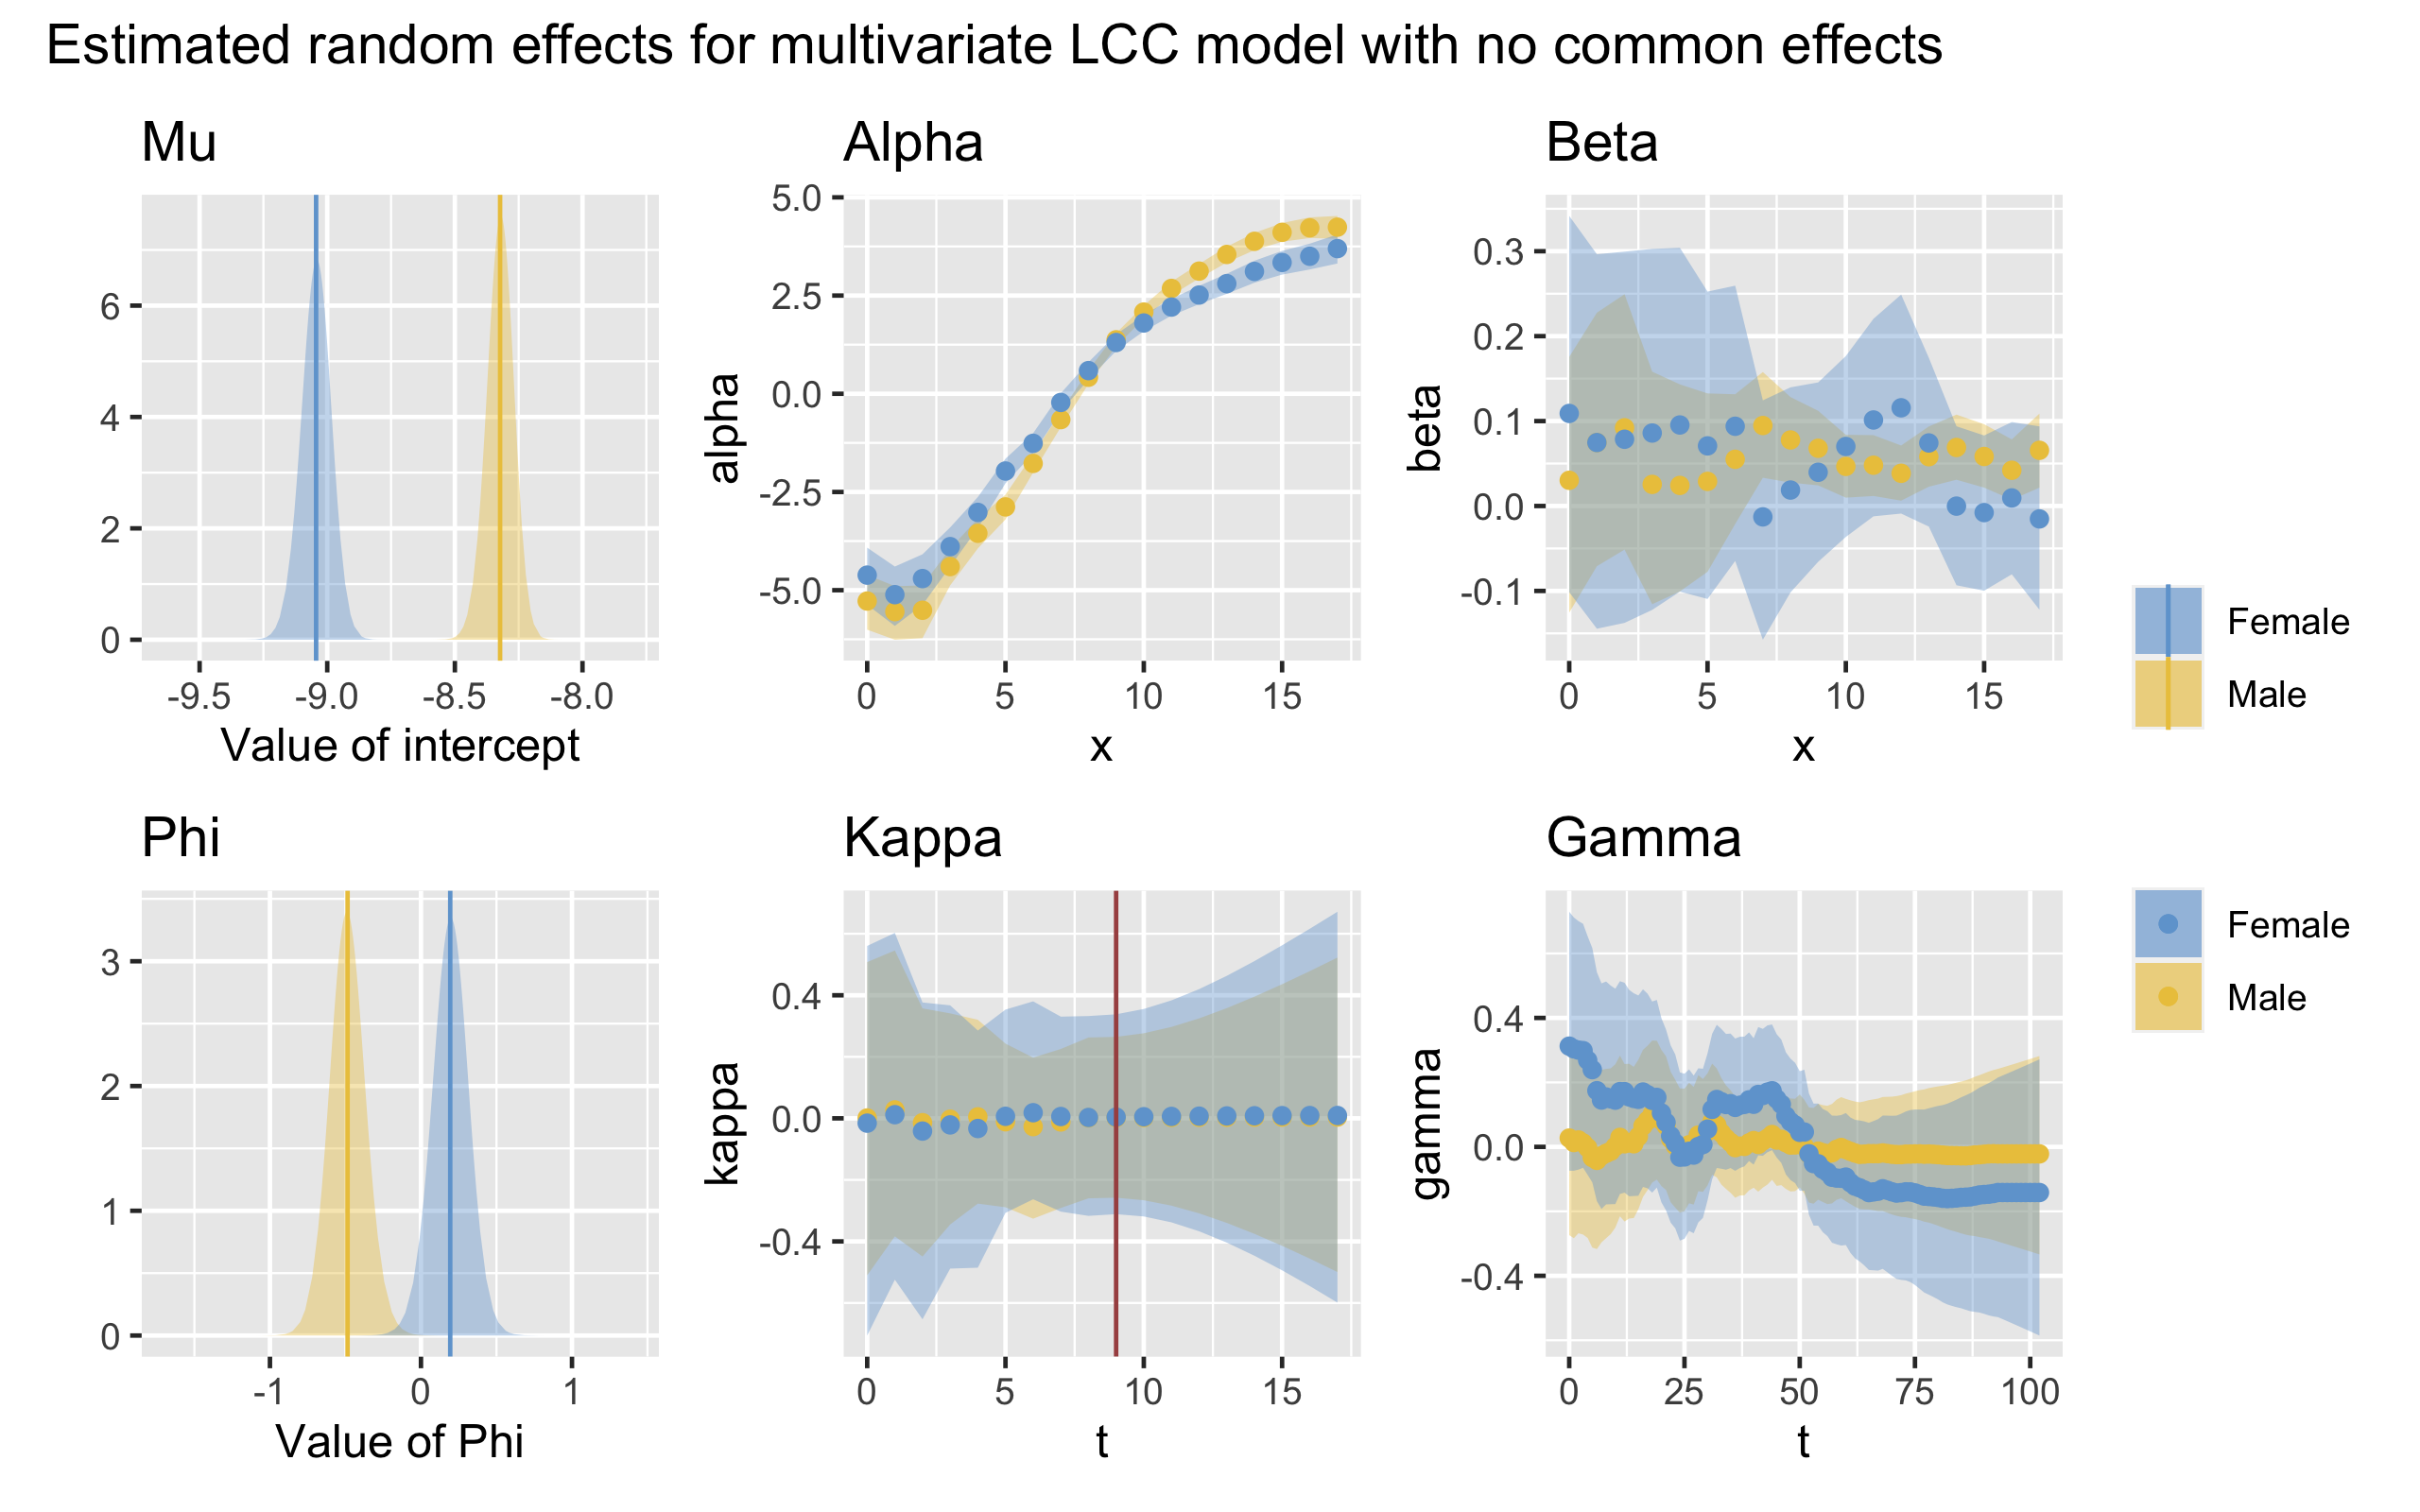
\includegraphics[width=\linewidth]{real-data/real-data-multivariate/Figures/effects-LCC-no-common-stomach.png}
        \caption{The estimated overall mortality level $\mu^{\text{sex}}$ and the estimated random effects $\alpha_x^{\text{sex}}$, $\beta_x^{\text{sex}}$, $\phi^{\text{sex}}$, $\kappa_t^{\text{sex}}$ and $\gamma_k^{\text{sex}}$ produced with inference with the "No common"-model.}
        \label{fig:effects-LCC-stomach-bottom}
    \end{subfigure}
    \caption{The mean values and the 95\% confidence bounds of the estimated random effects produced by inference with the "Common period" and the "No common" LCC-models on stomach cancer data. The layout of the plot is similar to that of e.g. Figure \ref{fig:uv-full-data-LC-l}. The effects that are modelled as common for male and female are plotted in green, and the effects that are modelled as specific to males and females are plotted in yellow and blue, respectively. The red line marks the beginning of the predicted period. }
    \label{fig:effects-LCC-stomach}
\end{figure}